\documentclass[12pt, twoside]{book}
\usepackage[utf8]{inputenc}
\usepackage[T1]{fontenc}
\usepackage[italian]{babel}
\usepackage{geometry}
\geometry{a4paper ,  top = 2.5 cm , bottom = 2.5 cm, left = 2.5 cm , right = 2.5 cm}


\usepackage{graphicx} 
\usepackage{amsmath}
\usepackage{amssymb}		% Required for inserting images
\usepackage{amsfonts}
\usepackage[most]{tcolorbox}
\usepackage{amsthm}
\usepackage{cancel}
\newcommand{\prodscal}[2]{\vec{#1} \cdot \vec{#2}}

\usepackage{changepage}
\usepackage{upgreek}
\usepackage{mathrsfs}
\usepackage{eufrak}
\usepackage{siunitx}
\usepackage{xcolor}
\usepackage{float}
\usepackage{textcomp}
\usepackage{comment}
\usepackage{titling}
\usepackage{parskip}
\usepackage{titlesec}
\usepackage{multicol}
%\usepackage{subfigure}
\usepackage{wrapfig}
\usepackage{caption}
\captionsetup{font=small}
\usepackage{subcaption}
\usepackage{listings}
\usepackage{color}
\usepackage{numprint}
\npthousandsep{\,}
\usepackage{enumerate}
\usepackage{fancyhdr}

\definecolor{codegray}{rgb}{0.5,0.5,0.5}
\definecolor{codepurple}{rgb}{0.58,0,0.82}

\usepackage{hyperref}
\hypersetup{
	colorlinks=true,
	linkcolor=blue,
	filecolor=magenta,      
	urlcolor=blue,
	pdftitle={},
	pdfpagemode=FullScreen,
}

\urlstyle{same}

% Definizione dell'intestazione per pagine dispari (Odd)
\fancyhead[LO]{\textbf{\thepage}}  % Numero di pagina in grassetto a sinistra
\fancyhead[RO]{\nouppercase\rightmark}         % Capitolo e sezione a destra

% Definizione dell'intestazione per pagine pari (Even)
\fancyhead[LE]{\nouppercase\leftmark}          % Capitolo e sezione a sinistra
\fancyhead[RE]{\textbf{\thepage}}  % Numero di pagina in grassetto a destra

% Cancella il footer
\fancyfoot{}
\setlength{\headheight}{14.49998pt}
\addtolength{\topmargin}{-2.49998pt}
% Personalizzazione della linea orizzontale
\renewcommand{\headrulewidth}{0.4pt}
\renewcommand{\footrulewidth}{0pt}

\setlength{\parindent}{0pt}
\addto\captionsitalian{\renewcommand*\figurename{\textsc{Fig.}}}
\addto\captionsitalian{\renewcommand*\tablename{\textsc{Tab.}}}


% PER IMPORTARE GLI SCRIPT
\usepackage{listings}

\definecolor{lstbg}{HTML}{F7F7F7}
\definecolor{lstframe}{HTML}{D9D9D9}
\definecolor{lstnumbers}{HTML}{808080}
\definecolor{lstkeyword}{HTML}{0000CC}
\definecolor{lstcomment}{HTML}{008000}
\definecolor{lststring}{HTML}{A31515}
\definecolor{lstidentifier}{HTML}{111111}
\definecolor{lstemph}{HTML}{795E26}

\lstdefinestyle{base}{
	backgroundcolor=\color{lstbg},
	basicstyle=\ttfamily\small\color{lstidentifier},
	keywordstyle=\bfseries\color{lstkeyword},
	commentstyle=\itshape\color{lstcomment},
	stringstyle=\color{lststring},
	showstringspaces=false,
	breaklines=true,
	breakatwhitespace=false,
	tabsize=4,
	captionpos=b,
	frame=single,
	rulecolor=\color{lstframe},
	framesep=6pt,
	framerule=0.8pt,
	numbers=left,
	numberstyle=\scriptsize\color{lstnumbers},
	stepnumber=1,
	numbersep=10pt,
	xleftmargin=20pt,
	framexleftmargin=20pt,
	xrightmargin=4pt,
	aboveskip=1.2em,
	belowskip=1.2em
}


\lstdefinestyle{Cstyle}{
	style=base,
	language=C,
	emph={printf,scanf,fprintf,fscanf,malloc,calloc,realloc,free,return,if,else,for,while,do,switch,case,break,continue},
	emphstyle=\color{red}\bfseries
}

\lstdefinestyle{Pythonstyle}{
	style=base,
	language=Python,
	emph={print,len,range,enumerate,zip,int,float,str,list,dict,set,tuple,input,open},
	emphstyle=\color{red}\bfseries
}

\lstdefinestyle{Fortranstyle}{
	style=base,
	language=Fortran,
	emph={program,end,subroutine,function,implicit,none,integer,real,double,precision,parameter,allocate,deallocate,print,write,read,do,if,then,else},
	emphstyle=\color{red}\bfseries
}



% Stile base per teoremi/definizioni
\tcbset{
	theobox/.style={
		enhanced,
		breakable,
		colback=gray!3!white,      % sfondo leggermente più scuro della pagina
		colframe=blue!60!black,     % bordo rosso scuro
		coltitle=blue!40!black,
		fonttitle=\bfseries,
		boxed title style={
			colback=blue!10!white,    % sfondo del titolo un po' più saturo
			boxrule=0.8pt
		},
		attach boxed title to top left={
			xshift=2mm,
			yshift=-2mm
		},
		top=3mm,
		bottom=3mm,
		left=3mm,
		right=3mm,
		separator sign={}
	}
}

% Teorema
\newtcbtheorem[no counter]{teorema}{}%
{theobox}{th}

% Definizione (stesso stile, titolo diverso)
\newtcbtheorem[no counter]{definizione}{Definizione}%
{theobox, breakable=false}{defnb}

% Approfondimenti (verde)
\newtcolorbox{approfondimento}[2][]{%
	enhanced,
	breakable,
	colback=white!5!white,
	colframe=blue!50!black,
	coltitle=blue!40!black,
	fonttitle=\bfseries,
	title={#2},
	boxed title style={
		colback=white!10!white,
		boxrule=0.8pt
	},
	attach boxed title to top left={
		xshift=2mm,
		yshift=-2mm
	},
	top=3mm,
	bottom=3mm,
	left=3mm,
	right=3mm,
	#1
}


% Dimostrazioni (grigio chiaro, testo più piccolo)
\newtcolorbox{dimostrazione}[2][]{%
	enhanced,
	breakable,
	colback=gray!5!white,
	colframe=gray!50!black,
	coltitle=black,
	fonttitle=\bfseries,
	fontupper=\small,            % testo dentro la dimostrazione in \small
	title={#2},
	boxed title style={
		colback=gray!15!white,
		boxrule=0.6pt
	},
	attach boxed title to top left={
		xshift=2mm,
		yshift=-2mm
	},
	top=2mm,
	bottom=2mm,
	left=3mm,
	right=3mm,
	#1
}


%
%%%%%%%%%%%%%%%%%%%%%%%%%%%%%%%%%%%%%%%%%%%%%%%%%%%%%%%%%%%%%%%%%%%%%
%%%%%%%%%%%%%%%%%%%%%%%%%%%%%%%%%%%%%%%%%%%%%%%%%%%%%%%%%%%%%%%%%%%%%
%%%%%%%%%%%%%%%%%%%%%%%%%%%%%%%%%%%%%%%%%%%%%%%%%%%%%%%%%%%%%%%%%%%%%
%
\title{Metodi numerici per la fisica: \\ l'arte della programmazione}
\author{Nicolò Mone}
%
%%%%%%%%%%%%%%%%%%%%%%%%%%%%%%%%%%%%%%%%%%%%%%%%%%%%%%%%%%%%%%%%%%%%%
%%%%%%%%%%%%%%%%%%%%%%%%%%%%%%%%%%%%%%%%%%%%%%%%%%%%%%%%%%%%%%%%%%%%%
%%%%%%%%%%%%%%%%%%%%%%%%%%%%%%%%%%%%%%%%%%%%%%%%%%%%%%%%%%%%%%%%%%%%%
%



%
%%%%%%%%%%%%%%%%%%%%%%%%%%%%%%%%%%%%%%%%%%%%%%%%%%%%%%%%%%%%%%%%%%%%%
%%%%%%%%%%%%%%%%%%%%%%%%%%%%%%%%%%%%%%%%%%%%%%%%%%%%%%%%%%%%%%%%%%%%%
%%%%%%%%%%%%%%%%%%%%%%%%%%%%%%%%%%%%%%%%%%%%%%%%%%%%%%%%%%%%%%%%%%%%%
%
\begin{document}
	
	
	\begin{titlepage}
		\centering
		\vspace*{3cm}
		{\huge\bfseries Appunti di metodi numerici \par}
		{\Large\bfseries l'arte della programmazione \par}
		\vspace{2cm}
		{\Large\itshape Nicolò Mone\par}
				
		\vfill
	\end{titlepage}
	\pagestyle{empty}
	\vspace*{\fill}
	Qui di solito ci va la common creative license ma chi ce l'ha e chi se ne fotte
	\cleardoublepage
	\vspace*{8cm}
	\begin{center}
		\begin{flushright}
			\small\emph{Qualcosa di commovente
			}
		\end{flushright}
		\vspace*{\fill}
	\end{center}
	\cleardoublepage
	\pagestyle{fancy}
	
	
	%
	%
	\chapter*{Introduzione}
	
	\addcontentsline{toc}{chapter}{Introduzione}
	
	\markboth{Introduzione}{Introduzione}
	
	\emph{Pisa, \today} \hfill Nicolò Mone
	
	
	%
	%
	\tableofcontents
	%
	%
	
	\newpage 
	
	\chapter{Numeri casuali}

\subsection{Introduzione}

In molte applicazioni di analisi numerica è necessario disporre di sequenze di numeri casuali. In realtà i computer non producono numeri casuali, generano sequenze \emph{pseudo-casuali}, cioè successioni determinate da algoritmi deterministici che imitano alcune proprietà statistiche della casualità.

In linea di principio esistono algoritmi che sfruttano sorgenti fisiche per produrre numeri "realmente" (?) casuali, ma nella maggior parte delle applicazioni numeriche si utilizzano generatori pseudo–casuali.

Un generatore di numeri casuali deve produrre sequenze che siano, almeno dal punto di vista statistico, il più possibile indipendenti. Poiché l'algoritmo che produce tali numeri è deterministico, l'obiettivo è costruire procedure che simulino bene il comportamento di una successione indipendente.

Un punto importante è che il grado di ``casualità'' richiesto dipende fortemente dall'applicazione. In alcune simulazioni fisiche o nei metodi Monte Carlo sono richieste proprietà statistiche molto rigorose.

Un riferimento classico sull'argomento è

\begin{quote}
	D. E. Knuth, \emph{Seminumerical Algorithms}, volume 2 di \emph{The Art of Computer Programming}, Addison-Wesley (1981).
\end{quote}

\paragraph*{Considerazioni sui generatori}
Quando si utilizza un generatore di numeri pseudo–casuali è sempre opportuno mantenere un atteggiamento critico nei confronti dei risultati prodotti. In altre parole, bisogna sempre controllare che il generatore non introduca correlazioni indesiderate o artefatti statistici.

Un criterio empirico utile è il seguente: se due generatori diversi producono risultati significativamente differenti per lo stesso esperimento numerico, è probabile che almeno uno dei due presenti problemi.

\begin{quote}
	\emph{``Be suspicious. Once you've been suspicious, stop and be suspicious again.''}\\
	\hfill - Riccardo Mannella
\end{quote}

\vspace{0.5cm}
\subsection{Generatori congruenziali lineari}

Uno dei generatori più elementari e diffusi è il \emph{linear congruential generator}. La sequenza viene costruita tramite la relazione ricorsiva:

\[
x_{n+1} = a x_n + c \pmod m .
\]

Qui $a$ è il moltiplicatore, $c$ è l'incremento, $m$ è il modulo. Scelti $a,\, c,\, m$ ed un '\emph{seed}' $x_n$, la sequenza è continua da sé in modo del tutto deterministico.

Questo tipo di generatore ha il vantaggio di essere molto veloce e di poter essere implementato con grande efficienza anche a basso livello.

Tuttavia presenta alcuni limiti importanti. Le sequenze generate possono mostrare correlazioni interne. Innanzitutto perché la successione può assumere solamente valori fra 0 ed $m-1$

In particolare, se si rappresentano graficamente i punti $(x_n, x_{n+1}, \dots, x_{n+k-1})$ in uno spazio $k$-dimensionale, si osserva che tali punti non riempiono uniformemente lo spazio, ma si dispongono su un insieme di iperpiani.

\begin{multicols}{2}

Più precisamente, i punti generati occupano uno spazio di dimensione $k-1$ e il numero massimo di tali piani è al più $m^{1/k}$, per questo si scelgono sempre alti valori di $m$ per non vedere la periodicità.

Per esempio, scegliendo $m = 2^{32}\,, \text{ e } k = 3\, ,$ si ottiene $m^{1/k}\, \approx\, 1600$ .

Altri esempi con $k=3$:
\begin{itemize}
	\item per $a=421\, ,\, c=1663\, ,\, \text{e } m=7875$, 100 punti e $m^{1/k}\, \approx\, 19.9$;
	\item per $a=4096\, ,\, c=150889\, ,\, \text{e } m=714025$, 10'000 punti e $m^{1/k}\, \approx\, 63.8$.
\end{itemize}

Questo significa che i punti tridimensionali generati dal metodo si dispongono su un numero relativamente limitato di piani, evidenziando quindi una struttura geometrica non desiderata nella sequenza pseudo–casuale.

\begin{figure}[H]
	\centering
	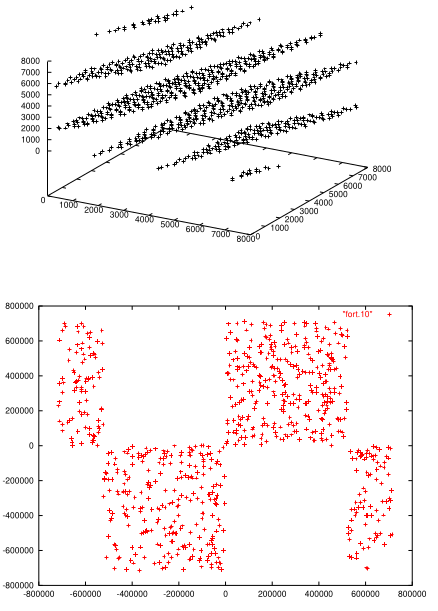
\includegraphics[width=6.5cm]{img/random1.png}
	\label{random 1}
	\caption{ Come si dispongono i punti della successione pseudo-casuale? si nota l'emergere di iperpiani affini che indicano correlazione statistica. La rappresentazione è tridimensionale perché $k=3$. Gli assi rappresentano i punti $(x_n, x_{n+1}, x_{n+3-1})$. }
\end{figure}

\end{multicols}

La rappresentazione grafica mostra chiaramente che i punti non riempiono uniformemente lo spazio tridimensionale, ma si dispongono su un insieme relativamente piccolo di piani.


\vspace{0.5cm}
\subsection{Combinazione di generatori}

Una possibile strategia per migliorare le proprietà statistiche dei generatori congruenziali consiste nel combinare più generatori tra loro.

Un esempio è la routine \texttt{RAN1.F}, che combina tre metodi congruenziali differenti. In particolare, vengono utilizzati generatori distinti per i bit più significativi, per quelli meno significativi e per una procedura di \emph{reshuffling} della sequenza.

Se la velocità di esecuzione è il fattore principale, è possibile utilizzare una combinazione più semplice di due generatori congruenziali. Questa strategia è adottata nella routine \texttt{RAN2}. Tuttavia, in questo caso il generatore tende a campionare una porzione più limitata dello spazio delle configurazioni.

\lstinputlisting[style=Fortranstyle,
	caption={RAN1.f90, combinazione di generatori congruenziali, esempio ispirato al \emph{"Numerical Recipes"} di Press, Teukolsky, Vetterling, Flannery. Nota bene: questa è solamente una routine, per essere utilizzata va chiamata},
	label={lst:combinazione generatori}]{RAN1.f90}


\vspace{0.5cm}
\subsection{Generatori basati su sistemi caotici}

Un approccio alternativo consiste nello sfruttare il comportamento caotico di alcuni sistemi dinamici.

L'idea è quella di utilizzare un sistema dinamico deterministico che presenti una dinamica caotica controllata, e impiegare la successione dei suoi stati come sequenza pseudo–casuale.

\begin{multicols}{2}

Un esempio classico è dato dalla mappa logistica:

\begin{equation}
	\label{logistic map eq}
	x_{n+1} = \lambda x_n (1 - x_n)\ \ .
\end{equation}

Al variare del parametro $\lambda$ il sistema in eq.(\ref{logistic map eq}) mostra un comportamento sempre più complesso, fino a entrare in regime caotico (come si vede in figura).


\begin{figure}[H]
	\centering
	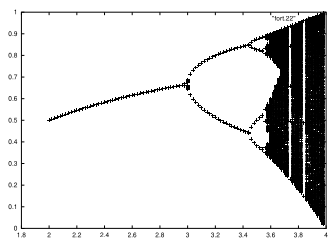
\includegraphics[width=6.5cm]{img/logisticcurve.png}
	\label{logistic map img}
	\caption{ La \href{https://youtu.be/ovJcsL7vyrk?si=zD5sAjndwQtBor5K}{curva logistica}, sembra di essere tornati a \href{https://youtu.be/j07YwnzGnII?si=a3Tg0EYx67gUO86X}{lezione da Paolini}, wow }
\end{figure}

\end{multicols}

Tuttavia l'utilizzo diretto di sistemi caotici come generatori pseudo–casuali presenta diversi problemi pratici. In particolare, è necessario stabilire quanto il comportamento caotico del sistema sia effettivamente adeguato per simulare una sequenza statisticamente indipendente.


\vspace{0.5cm}
\subsection{Generatori come sistemi dinamici a molti stati}

Un modo più efficace per costruire generatori pseudo–casuali consiste nel progettare sistemi dinamici con un numero elevato di stati interni.

L'idea è quella di costruire una macchina a molti stati in cui il valore successivo della sequenza dipende da una combinazione di stati precedenti. Questo schema può essere rappresentato come una rete di variabili interne che interagiscono tra loro attraverso operazioni di somma o sottrazione.

Questa idea è alla base dei cosiddetti algoritmi \emph{add and carry} oppure \emph{subtract and carry}. Tra i generatori di questo tipo si trovano, ad esempio,

\begin{itemize}
	\item la routine \texttt{RAN3}: si mantiene una tabella di numeri precedenti e si genera il nuovo valore come differenza di due elementi della sequenza (In forma semplificata: $x_n=x_{n−j}-x_{n−k}$);
	
	\item il generatore \texttt{rcarry}: questo è un generatore della famiglia subtract-with-carry. È simile a quello precedente ma introduce una variabile aggiuntiva chiamata carry (l'idea è: $x_n=x_{n−r}-x_{n−s}-c$).
\end{itemize}

Questi algoritmi presentano in genere periodi di ripetizione molto lunghi e buone proprietà statistiche (risolvendo parzialmente il problema della struttura geometrica in iperpiani).




\section{Generazione di distribuzioni non uniformi}

\subsection{Dal caso uniforme a una distribuzione arbitraria}

Dopo aver costruito un generatore di numeri pseudo--casuali uniformi, il problema successivo consiste nel produrre variabili aleatorie con una distribuzione assegnata. In altre parole, dato un generatore che fornisce variabili uniformi, vogliamo ottenere campioni distribuiti secondo una densità prefissata.

Sia dunque $x$ una variabile casuale distribuita uniformemente in un certo intervallo, con densità $p(x)$, e supponiamo di voler costruire una nuova variabile $y$ con densità $p(y)$. La relazione fondamentale tra le due densità si ottiene imponendo l'\underline{invarianza della probabilità} sotto trasformazione di variabile.
Si ha infatti $|p(y)\,dy| = p(x)\,dx$, da questa relazione segue immediatamente che:

\[
p(y) = p(x)\left|\frac{dx}{dy}\right| .
\]

Questa formula esprime il fatto che la densità della nuova variabile dipende dalla densità di partenza e dal modo in cui la trasformazione $x \mapsto y$ dilata o contrae gli intervalli.

Il problema centrale diventa allora quello di determinare una trasformazione opportuna tra $x$ e $y$. Ciò si riconduce a risolvere
$\frac{dx}{dy} = f(y)$ .

In sostanza, assegnata la distribuzione voluta, si cerca una funzione di trasformazione tale che la variabile uniforme iniziale venga mappata nella nuova variabile con la densità desiderata.

%
%
%
\vspace{0.5cm}
\subsection{Metodo della funzione cumulativa inversa}

Il procedimento precedente si chiarisce riscrivendo la trasformazione in termini di funzione integrale della densità.

Ricordando la relazione $\frac{dx}{dy} = f(y)$ ed integrando rispetto a $y$, si ottiene

\[ x = F(y)\ \ ,\]

dove la funzione $F(y)$ è data, a meno di costanti additive o di opportune normalizzazioni, dall'integrale della densità:

\[ F(y) = \int p(y)\,dy\ \ . \]

Se la funzione $F$ è invertibile, allora si può esprimere $y$ in funzione di $x$ come

\[
y(x) = F^{-1}(x).
\]

Questo è il contenuto essenziale del metodo della trasformazione inversa: si genera una variabile uniforme $x$, si costruisce la funzione cumulativa associata alla densità desiderata, e infine si ottiene la variabile distribuita secondo $p(y)$ applicando l'inversa della cumulativa.

Il metodo funziona quindi molto bene quando l'inversa dell'integrale di $p(y)$ è disponibile in forma esplicita, oppure può essere calcolata numericamente in modo efficiente. 




\subsubsection{Esempio: distribuzione esponenziale}

Un esempio particolarmente importante è quello della distribuzione esponenziale. Si consideri la trasformazione

\[
y(x) = -\ln x .
\]

Se $x$ è uniforme nell'intervallo $(0,1)$, allora

\[
\frac{dx}{dy} = -e^{-y},
\qquad
\left|\frac{dx}{dy}\right| = e^{-y}.
\]

Poiché la densità di $x$ è uniforme, cioè costante su $(0,1)$, dalla relazione generale

\[
p(y)\,dy = p(x)\left|\frac{dx}{dy}\right|dy
\]

segue che, a meno della costante uniforme $p(x)$, la densità di $y$ è

\[
p(y)\,dy = e^{-y}\,dy .
\]

Si ottiene dunque la distribuzione esponenziale. 


%
%
%
\subsubsection{Interpretazione geometrica del metodo}

Ripartiamo da $F(y) = \int p(y)\,dy$ ; si osserva che la variabile uniforme $x$ viene ottenuta come valore della cumulativa associata a $y$. Invertendo questa relazione, si ha ancora

\[
y(x) = F^{-1}(x).
\]

Geometricamente, la funzione $F(y)$ cresce dal valore minimo al valore massimo della probabilità cumulata. Se si estrae un numero uniforme $x$ tra $0$ e $1$, lo si può interpretare come un livello di probabilità cumulata; il valore corrispondente di $y$ si ottiene leggendo sull'asse orizzontale il punto in cui la cumulativa raggiunge proprio quel livello.

In altre parole, il metodo della trasformazione inversa trasforma una distribuzione uniforme della probabilità cumulata in una distribuzione non uniforme della variabile fisica.

\subsubsection{Esempio: tempi di decadimento}

Sappiamo che quando i nuclei decadono hanno una densità di probabilità $p(t)\,=\, \lambda e^{-\lambda \, t}$ di decadere, nel senso che $p(t)\,dt$ è la probabilità di decadere nell'intervallo di tempo $t$, $t+dt$; inoltre sappiamo che la cumulativa di questa probabilità, 
\[F(t^*)\,=\, P(T<t^*)\,=\, \int_0^{t^*} p(T)\, dT\,=\, 1-e^{-\lambda \, t^*}\]
ci dà invece la probabilità che il nucleo sia decaduto prima dell'istante $t^*$.

Partiamo quindi dalla probabilità accumulata ed scegliamo un valore $u\in[0,\, 1]$, per poi porre l'uguaglianza $1-e^{-\lambda \, t^*}=u$ che invertita restituisce $t^*=-\frac{1}{\lambda}\, \log(1-u)$. Questo passaggio equivale ad estrarre una percentuale di nuclei decaduti e a chiedersi 'quanto tempo $t^*$ si dovrebbe aspettare per vedere una frazione $u$ di nuclei decadere?'.

Nonostante il processo sia poissoniano ed ogni atomo decada dopo un tempo diverso, si può continuare ad estrarre valori $u$ quanti sono gli atomi e questo ci permette trovando tutti i tempi corrispondenti di ricostruire la distribuzione esponenziale iniziale.

%
%
%
\vspace{0.5cm}
\subsection{Trasformazioni in più dimensioni}

Il metodo di trasformazione non è limitato al caso unidimensionale, ma si estende anche a distribuzioni in più variabili.

Se $(x_1,x_2,\dots)$ è un vettore di variabili di partenza e $(y_1,y_2,\dots)$ è il nuovo vettore di variabili, allora la relazione tra le densità è regolata dal determinante jacobiano della trasformazione:

\[
p(y_1,y_2,\dots)\,dy_1dy_2\cdots
=
\left|
\frac{\partial(x_1,x_2,\dots)}{\partial(y_1,y_2,\dots)}
\right|
p(x_1,x_2,\dots)\,dy_1dy_2\cdots .
\]

Questa espressione generalizza direttamente la formula unidimensionale.

Anche qui il significato è lo stesso: la densità si modifica in funzione della deformazione locale dei volumi elementari operata dalla trasformazione.


\vspace{0.5cm}
\subsection{Generazione di distribuzioni gaussiane: metodo di Box-Muller}

Un'applicazione molto importante del caso multidimensionale è la generazione di variabili gaussiane: il metodo di \href{https://www.taygeta.com/random/gaussian.html}{Box-Muller}, che permette di ottenere due variabili gaussiane indipendenti a partire da due variabili uniformi indipendenti.

Si considerino due variabili uniformi indipendenti $x_1$ e $x_2$, entrambe distribuite uniformemente in $(0,1)$. Si definiscono allora le nuove variabili

\[
y_1 \,=\, \sqrt{-2\ln x_1}\,\cos(2\pi x_2) \,=\, r\cos\theta,
\]

\[
y_2 \,=\, \sqrt{-2\ln x_1}\,\sin(2\pi x_2) \,=\, r\sin\theta.
\]

Queste formule costituiscono la trasformazione di Box--Muller. Le due variabili uniformi $x_1$ e $x_2$ vengono reinterpretate come variabili ausiliarie che costruiscono, rispettivamente, il raggio e l'angolo in coordinate polari nel piano delle variabili gaussiane. In particolare, $r = \sqrt{-2\ln x_1}$ e $\theta = 2\pi x_2$ .

Questa trasformazione è progettata in modo tale che la densità congiunta di $(y_1,y_2)$ risulti gaussiana e radialmente simmetrica, così da avere una routine che trasformi due variabili indipendenti distribuite uniformemente in due variabili distribuite gaussianamente.

\begin{figure}[H]
	\centering
	\label{box-muller}
	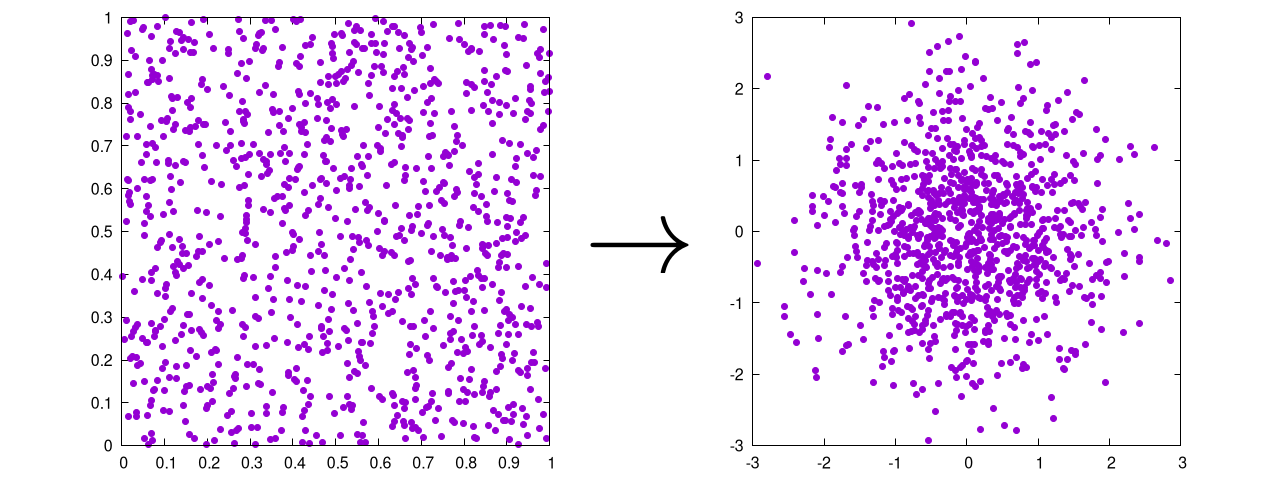
\includegraphics[width=10cm]{img/cartesian_rand_transform.png}
	\caption{Immagine presa da \href{https://www.algorithm-archive.org/contents/box_muller/box_muller.html}{QUI  <--}}
\end{figure}


\paragraph{Calcolo del Jacobiano nella trasformazione di Box-Muller}

Per giustificare il metodo bisogna analizzare lo jacobiano della trasformazione. Partiamo dalla trasformazione sopra presentata, con definizioni di $y_1,\, y_2,\, r,\, \theta$. Si ricava:

\[
x_1 = e^{-r^2/2},
\qquad
x_2 = \frac{\theta}{2\pi}.
\]

Poiché $x_1$ e $x_2$ sono uniformi e indipendenti, la loro densità congiunta è costante nel quadrato unitario: $p(x_1,x_2)=1,
\quad 0<x_1<1,\ 0<x_2<1$.


Ora, il passaggio da $(x_1,x_2)$ a $(r,\theta)$ produce il fattore jacobiano

\[\left|
\begin{matrix}
	\displaystyle\frac{\partial x_1}{\partial r} & \displaystyle\frac{\partial x_1}{\partial \theta}\\[4pt]
	\displaystyle\frac{\partial x_2}{\partial r} & \displaystyle\frac{\partial x_2}{\partial \theta}
\end{matrix}
\right|\ =\ 
\left|
\begin{matrix}
	-r e^{-r^2/2} & 0\\[4pt]
	0 & \frac{1}{2\pi}
\end{matrix}
\right|.\]

si ottiene $\displaystyle\left|\frac{\partial(x_1,x_2)}{\partial(r,\theta)}\right|\,=\,\displaystyle\frac{r}{2\pi}\, e^{-r^2/2}$ .


Per passare poi da coordinate polari a coordinate cartesiane si usa il noto elemento di area $dy_1\,dy_2 = r\,dr\,d\theta$, cioè $dr\,d\theta = \displaystyle\frac{1}{r}\,dy_1\,dy_2$.

Combinando i due passaggi, si trova che la densità di $(y_1,y_2)$ è proporzionale a $\displaystyle\frac{r}{2\pi}e^{-r^2/2}\cdot \frac{1}{r}\, =\,\displaystyle\frac{1}{2\pi}e^{-r^2/2}$.
Poiché $r^2 = y_1^2 + y_2^2$, segue che:

\[
P(y_1,y_2)=\frac{1}{2\pi}\exp\left(-\frac{y_1^2}{2}-\frac{y_2^2}{2}\right).
\]

Questa è precisamente la distribuzione normale bidimensionale standard 
con componenti indipendenti.

%
%
%
%\vspace{0.5cm}
\subsubsection{Osservazione conclusiva su questa parte}

Riassumendo, il principio generale è il seguente: una volta ottenute variabili uniformi affidabili, si possono costruire distribuzioni non uniformi applicando trasformazioni opportune. Nel caso unidimensionale il punto chiave è l'inversione della cumulativa; nel caso multidimensionale entra in gioco il determinante jacobiano della trasformazione.

Questo quadro teorico prepara direttamente al metodo di \emph{rejection}, che diventa essenziale quando l'inversa della cumulativa non è disponibile in forma trattabile.

%
%
%
\vspace{0.5cm}
\section{Rejection method}

Il metodo del rifiuto permette di generare distribuzioni non uniformi senza richiedere il calcolo esplicito dell'integrale della densità.

Si consideri una distribuzione di probabilità desiderata $p(x)$, e una funzione $f(x)$ tale che $f(x) > p(x) \quad \forall\ x$ , l'idea è utilizzare una coppia di variabili casuali uniformi per campionare la distribuzione $p(x)$.

Si procede nel seguente modo:

\begin{itemize}
	\item si estrae un valore $x_s$ uniformemente distribuito nel dominio;
	\item si estrae una seconda variabile casuale $x_1$ uniforme tra $0$ e $f(x_s)$;
	\item si accetta $x_s$ se vale la condizione $x_1 < p(x_s)$
\end{itemize}

Se la condizione non è soddisfatta, il punto viene rifiutato e si ripete la procedura. Questo metodo non richiede la conoscenza della funzione cumulativa, ma soltanto una funzione $f(x)$ che sovrastimi $p(x)$.

\paragraph{Interpretazione geometrica:}

Il metodo può essere interpretato geometricamente. Si consideri il grafico delle funzioni $p(x)$ e $f(x)$, con $f(x)$ tale che $f(x) \ge p(x)$

\begin{multicols}{2}
\begin{figure}[H]
	\label{rejection img}
	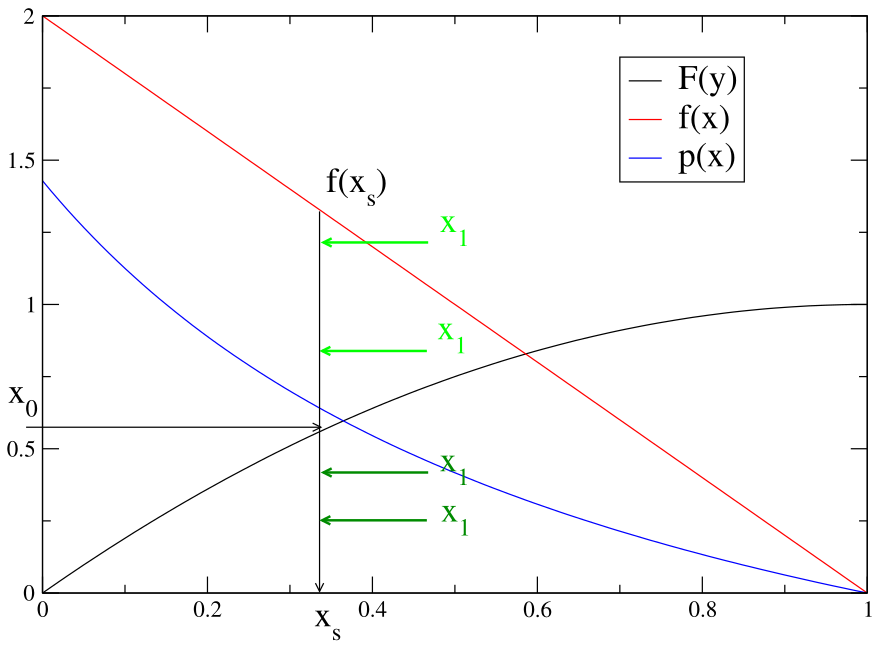
\includegraphics[width=6.9cm]{img/rejection.png}
	\caption{rappresentazione grafica del \emph{rejection method}}
\end{figure}

Si generano punti uniformemente nella regione delimitata da $f(x)$.

Un punto viene accettato se cade sotto la curva $p(x)$.

In questo modo, i punti accettati risultano distribuiti secondo la densità desiderata.

In fig.(\ref{rejection img}), i punti accettati sono quelli che cadono sotto $p(x)$, mentre gli altri vengono scartati.
\end{multicols}

%
%
%
\subsection{Metodo del rifiuto per la distribuzione Gamma}

La distribuzione Gamma di ordine intero $a > 0$ rappresenta la distribuzione del tempo di attesa per il verificarsi del $a$-esimo evento in un processo di Poisson con valore medio unitario ed è data da:

\begin{equation}
	p_a(x)\,dx \ =\
	\frac{x^{a-1} e^{-x}}{\Gamma(a)}\,dx\ \ ,
	\qquad x>0\ \ ,
\end{equation}


Per valori piccoli di $a$, è possibile generare direttamente la distribuzione come somma di variabili esponenziali indipendenti.

Questo equivale a calcolare il prodotto di $a$ variabili casuali uniformi e successivamente prendere il logaritmo.

Per valori più grandi di $a$, la distribuzione assume una forma a campana: con massimo circa in $x \approx a$ e larghezza dell'ordine $\sqrt{a}$

%
\subsubsection{Funzione di confronto}

Per applicare il metodo del rifiuto, si introduce una funzione di confronto.

Una scelta conveniente che si rivela utile è la distribuzione di Lorentz:

\begin{equation}
	\label{Lorentziana}
	p(y)\,dy =
	\frac{1}{\pi (1 + y^2)}\,dy
\end{equation}

Integrandola si ottiene

\begin{equation}
	F(y) = \int p(y)\,dy = \frac{1}{\pi} \arctan(y)
\end{equation}

\begin{multicols}{2}
	
%
\subsubsection{Funzione di maggiorazione}

Si introduce una funzione $f(x)$ della forma

\begin{equation}
	f(x)\ =\
	\frac{c_0}{1\, +\, (x - x_0)^2 / a_0^2}
\end{equation}

Questa funzione deve essere scelta in modo tale che $f(x) \ge p(x)$ e che il prodotto $a_0\, c_0$ sia il più piccolo possibile, al fine di minimizzare il numero di rifiuti.

\begin{figure}[H]
	\centering	
	\label{gamma+lorentz}
	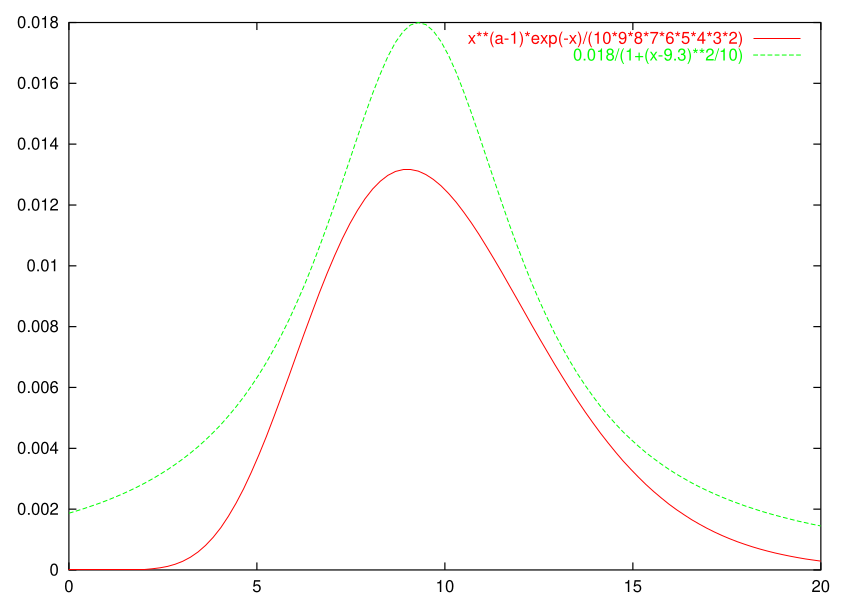
\includegraphics[width=6cm]{img/gamma_function.png}
	\caption{\emph{Gamma function} in rosso, mentre in verde si vede la lorentziana, funzione di maggiorazione $f(x)$.}
\end{figure}
\end{multicols}

\subsubsection{Algoritmo}

Si genera una variabile uniforme $u \in [0,1]$ e si pone $x = a_0 \tan(\pi u) + x_0$ cioè $x = f^{-1}(y)$.

Successivamente si verifica la condizione di accettazione (rejection test).

Questo procedimento è implementato, ad esempio, nella routine \texttt{GAMDEV}.

\lstinputlisting[style=Cstyle,
	caption={Implementazione del metodo GAMDEV},
	label={lst:gamma rejection}]{GAMDEV.c}


%
%
%
\vspace{0.5cm}
\section{Integrazione Monte Carlo}

Il metodo di integrazione Monte Carlo è strettamente collegato al metodo del rifiuto.

Esso permette di stimare integrali multidimensionali mediante campionamento casuale.

In uno spazio $n$-dimensionale, dato un insieme di $N$ punti $x_i$, vale la stima

\begin{equation}
	\int_V f\,dV\ \approx\ V \langle f \rangle\, \pm\, V\, \sqrt{\frac{\langle f^2 \rangle - \langle f \rangle^2}{N}}
\end{equation}

dove

\begin{equation}
	\langle f^n \rangle =
	\frac{1}{N} \sum_{i=1}^N f^n(x_i)
\end{equation}

\begin{multicols}{2}
\subsubsection{Interpretazione}

L'idea è quella di incorporare una regione difficile da campionare all'interno di una regione più semplice, dalla quale è possibile estrarre punti uniformemente.

Successivamente si utilizza il campionamento casuale per stimare l'integrale.

Il metodo può essere scritto in molti modi diversi in base a in quante dimensioni stiamo campionando, in quale spazio estraiamo i nostri punti e che forma ha la funzione, ma il concetto rimane sempre questo.

\begin{figure}[H]
	\centering
	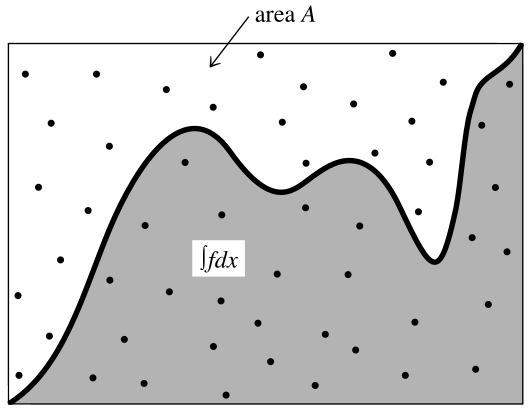
\includegraphics[width=7cm]{img/MonteCarloIntegration.png}
	\label{monte carlo}
	\caption{Esempio visuale preso da "\emph{Numerical Recipes in C}". L'integrale della funzione $f$ è stimato come l'area del rettangolo A moltiplicata per la frazione di punti che si trova sotto la curva $f$}
\end{figure}

\end{multicols}


\subsubsection{Esempio: area di un cerchio}

Si consideri il calcolo dell'area di un cerchio unitario.

Si definisce una funzione

\begin{equation}
	f =
	\begin{cases}
		1 & \text{all'interno del cerchio} \\
		0 & \text{all'esterno}
	\end{cases}
\end{equation}

Il volume della regione di campionamento è V = 4, la stima dell'area è $\int_V f\,dV \approx V \langle f \rangle$


\begin{multicols}{2}
Per $N = 1000$ si ottiene

\[\begin{aligned}
	\langle f \rangle &=\ 0.797\\
	\text{area} &=\ 3.19 \pm 0.05
\end{aligned}\]

Per $N = 10^6$:

\[\begin{aligned}
	\langle f \rangle &=\ 0.78616\\
	\text{area} &=\ 3.145 \pm 0.005
\end{aligned}\]

\begin{figure}[H]
	\centering
	\label{aa}
	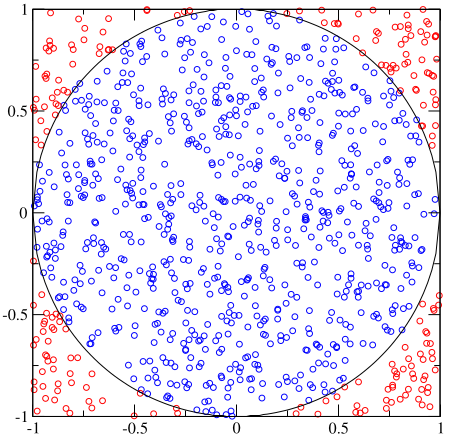
\includegraphics[width=5cm]{img/pie.png}
	\caption{Integrale Monte Carlo dell'area di un cerchio}
\end{figure}
\end{multicols}

%
\subsubsection{Esempio: disco con foro}

Si consideri un disco di raggio 1 con un foro di raggio 0.5 centrato nel punto $(0.5,0)$.

Si vogliono calcolare:

\begin{equation}
	x_{cm} = \frac{\int x\,dV}{\int dV}
\end{equation}

\begin{equation}
	I_{0,0} = \int (x^2 + y^2)\,dV
\end{equation}


\begin{multicols}{2}

Le funzioni da integrare sono:

\begin{itemize}
	\item $f_x = x$ all'interno della regione, zero fuori;
	\item $f_y^2 = y^2$, ecc.
\end{itemize}

Per $N = 10^6$ si ottiene:

\[\begin{aligned}
	x_{cm} &=\ -0.393\ \pm\ 0.004\\
	y_{cm} &=\ -0.000\ \pm\ 0.005\\
	I_{0,0} &\approx\ 1.275
\end{aligned}\]

\begin{figure}[H]
	\centering
	\label{aaa}
	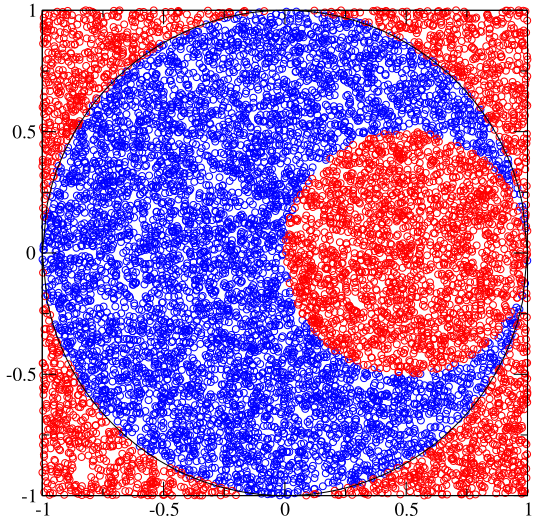
\includegraphics[width=6cm]{img/MCintegral.png}
	\caption{Integrale Monte Carlo dell'area di un cerchio forato}
\end{figure}
\end{multicols}

\lstinputlisting[style=Pythonstyle,
	caption={Esercizio di integrazione Monte Carlo del disco bucato in Python, scritta da ChatGpt 5.3},
	label={lst:gamma rejection}]{MonteCarloIntegration-HoledDisk.py}

	
	\newpage 
	
	\chapter{Ricerca degli zeri di una funzione}

\section{Introduzione}

La determinazione degli zeri di una funzione, ovvero la risoluzione dell'equazione $f(x) = 0$, costituisce uno dei problemi fondamentali dell'analisi numerica. Nonostante la formulazione apparentemente semplice, si tratta in generale di un problema non banale quando non si ha una soluzione analitica.

L'idea di base è la seguente: si cerca inizialmente di individuare in maniera approssimata una regione dello spazio in cui è presente uno zero della funzione; successivamente si utilizza un algoritmo numerico per raffinare progressivamente la stima.


\paragraph{Esempio introduttivo:}

\begin{multicols}{2}
Consideriamo la funzione

\[
f(x) = x + \frac{x^2}{10},
\]

e supponiamo di studiarla nell'intervallo

\[
[-15,\,10].
\]

Un primo approccio consiste nel valutare la funzione in un numero finito di punti (ad esempio 30 punti equispaziati) e osservare il comportamento del grafico. 

\begin{figure}[H]
	\centering
	\label{es1}
	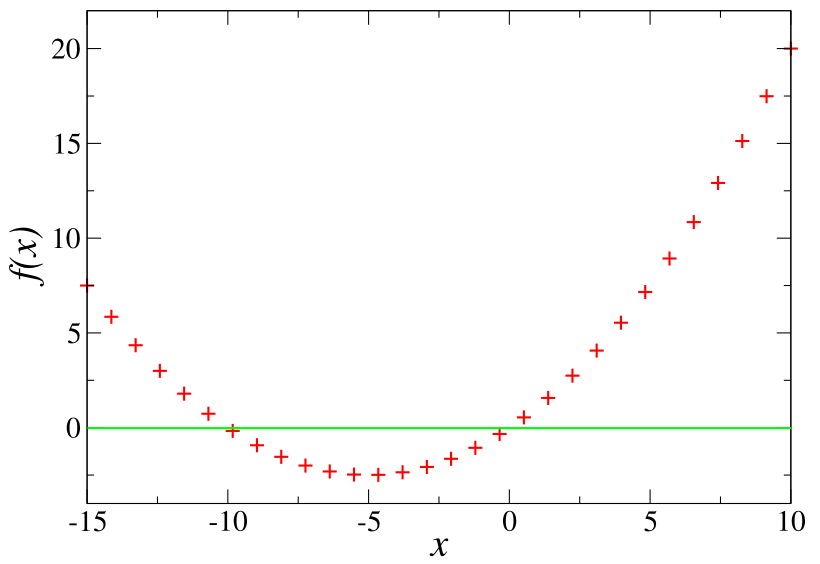
\includegraphics[width=7.2cm]{img/roots1.png}
	\caption{esempio di funzione $f(x)$ plottata con soli 30 punti per stimare i segmenti in cui cercare lo zero.}
\end{figure}

\end{multicols}

Questo permette di individuare visivamente la regione in cui la funzione cambia segno, e quindi dove è presente uno zero.

Questa fase preliminare è essenziale: senza una buona stima iniziale della posizione dello zero, molti metodi numerici risultano inefficaci o addirittura divergenti.

\paragraph{Casi difficili e comportamenti patologici:}

Esistono tuttavia funzioni per le quali la localizzazione dello zero può risultare estremamente complicata dal punto di vista numerico.

\begin{multicols}{2}
Un esempio significativo è dato dalla funzione

\[
f(x)\ =\ 3x^2\, +\, 1\, +\, \frac{\ln\left[(\pi - x)^2\right]}{\pi^4}.
\]

In questo caso esistono due zeri situati approssimativamente in

\[
x\ \approx\ \pi\, \pm\, 10^{-667}.
\]

\begin{figure}[H]
	\centering
	\label{es2}
	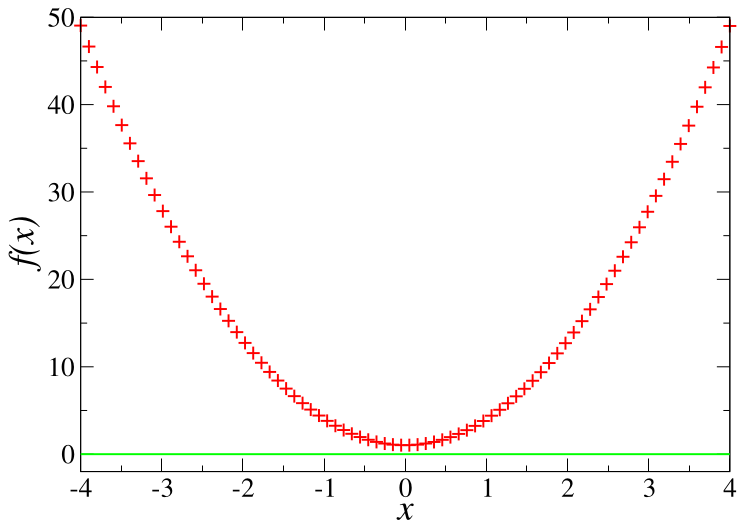
\includegraphics[width=7cm]{img/roots2.png}
	\caption{Funzione $f(x)$ plottata con 80 punti nel range [-4; 4]}
\end{figure}

\end{multicols}

Si tratta di zeri estremamente vicini al valore \( \pi \), tanto che una loro individuazione diretta tramite semplice campionamento risulta praticamente impossibile.

Tuttavia, osservando la struttura della funzione, si nota che il termine logaritmico diventa molto grande e negativo quando \( x \) si avvicina a \( \pi \). Questo suggerisce che lo zero si trovi nelle vicinanze di tale punto.

Questo esempio mostra chiaramente come, in molti casi, sia necessario combinare osservazioni qualitative sulla funzione con tecniche numeriche.

Nel seguito assumeremo di essere riusciti a individuare un intervallo che contiene uno zero della funzione e ci concentreremo su come raffinarne la posizione.

\section{Metodo di bisezione}

Una volta individuato un intervallo in cui è presente uno zero, il metodo più semplice per determinarlo con precisione è il \textbf{metodo di bisezione}.

Questo metodo si basa su una proprietà fondamentale delle funzioni continue: se una funzione cambia segno in un intervallo, allora deve necessariamente annullarsi in almeno un punto interno.

\paragraph{Idea del metodo}

Supponiamo di conoscere due punti \( x_1 \) e \( x_2 \) tali che la funzione cambia segno nell'intervallo \([x_1, x_2]\), ovvero:

\[
f(x_1) > 0, \qquad f(x_2) < 0,
\]

Si definisce quindi il punto medio $x_m = \frac{x_1 + x_2}{2}$ e si valuta il segno della funzione nello stesso:

\begin{itemize}
	\item se \( f(x_m) > 0 \), lo zero si trova nell'intervallo \([x_m, x_2]\), quindi si pone \( x_1 = x_m \);
	\item se \( f(x_m) < 0 \), lo zero si trova nell'intervallo \([x_1, x_m]\), quindi si pone \( x_2 = x_m \).
\end{itemize}

Il procedimento viene quindi iterato, restringendo progressivamente l'intervallo che contiene lo zero.

\paragraph{Stima dell'errore: }

Se inizialmente la lunghezza dell'intervallo è $\epsilon = |x_1 - x_2|$, dopo $n$ iterazioni la lunghezza dell'intervallo si riduce a $\delta \,\approx\,\epsilon\,/\,2^n$.

Questo fornisce una stima diretta dell'errore sulla posizione dello zero.

\paragraph{Esempio numerico del metodo di bisezione: }

Consideriamo la funzione

\[
f(x) = \frac{x^3}{5} + \frac{x}{5} + 0.1.
\]

Applicando il metodo di bisezione si ottiene la seguente sequenza di approssimazioni:

\begin{center}
	\begin{tabular}{c c c}
		\hline
		$i$ & $x_r$ & $\delta$ \\
		\hline
		1 & -0.9   & 0.9  \\
		2 & -0.45  & 0.45 \\
		3 & -0.23  & 0.23 \\
		4 & -0.338 & 0.11 \\
		5 & -0.394 & 0.06 \\
		6 & -0.422 & 0.03 \\
		\hline
	\end{tabular}
\end{center}

Si osserva come l'intervallo contenente lo zero si restringa progressivamente e la stima della radice converga.

\bigskip

Questo esempio illustra chiaramente il comportamento del metodo: la convergenza è garantita, ma relativamente lenta, poiché l'errore si riduce esponenzialmente con fattore \(1/2\) ad ogni iterazione.

\subsection{Osservazioni sul metodo di bisezione}

Il metodo di bisezione è estremamente robusto e presenta alcune caratteristiche fondamentali, esso converge purché la funzione sia continua e si riesca a individuare un intervallo in cui essa cambia segno. Tuttavia, la convergenza è relativamente lenta, in quanto l'errore si riduce secondo la legge $ \delta\, =\, \epsilon/2^n$. 

\begin{multicols}{2}
	
	\begin{figure}[H]
		\centering
		\label{zeri}
		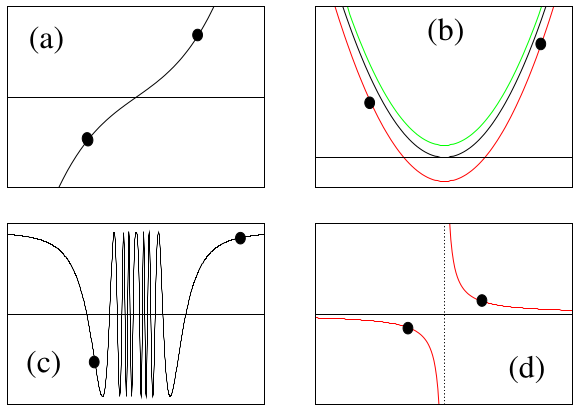
\includegraphics[width=7cm]{img/roots14.png}
		\caption{Casi particolari che si possono verificare.}
	\end{figure}
	
	Esistono diversi casi particolari che è opportuno considerare:
	
	\begin{itemize}
		\item \textbf{Caso normale}: la funzione cambia segno una sola volta nell'intervallo e il metodo converge allo zero corretto.
		\item \textbf{Radici multiple}: la funzione può toccare l'asse senza cambiare segno; in questo caso il metodo può non individuare correttamente lo zero.
		\item \textbf{Radici molto vicine}: possono esistere più zeri estremamente vicini tra loro, rendendo difficile l'identificazione numerica.
		\item \textbf{Discontinuità}: se la funzione presenta una discontinuità, il metodo converge comunque, ma al punto di discontinuità anziché a uno zero reale.
	\end{itemize}
	
	
\end{multicols}


%
%
%
\section{Metodo di Newton-Raphson}

Un approccio più sofisticato per il raffinamento della radice è il metodo di \textbf{Newton-Raphson}: supponiamo di avere una stima iniziale \( x \) della radice e di voler trovare una stima migliorata \( x_r \). Si approssima la funzione tramite lo sviluppo di Taylor al primo ordine:

\[
f(x_r)\ \approx\ f(x)\, +\, (x_r - x)\, \frac{df(x)}{dx} \ \overset{!}{=}\ 0\ \ .
\]

Imponendo la condizione \( f(x_r) \overset{!}{=} 0 \), da cui segue immediatamente

\begin{equation}
	\label{Newton-Raphson}
	x_r\ =\ x\, -\, \frac{f(x)}{f'(x)}.
	\quad \Rightarrow \quad 
	x_{i+1}\ =\ x_i\, -\, \frac{f(x_i)}{f'(x_i)}\ \ .
\end{equation}

Questa relazione definisce una procedura iterativa.

\paragraph{Esempio numerico: }

Consideriamo nuovamente la funzione $f(x) = \frac{x^3}{5} + \frac{x}{5} + 0.1\  .$

\begin{multicols}{2}
	
	\begin{figure}[H]
		\centering
		\label{NewtonCotes}
		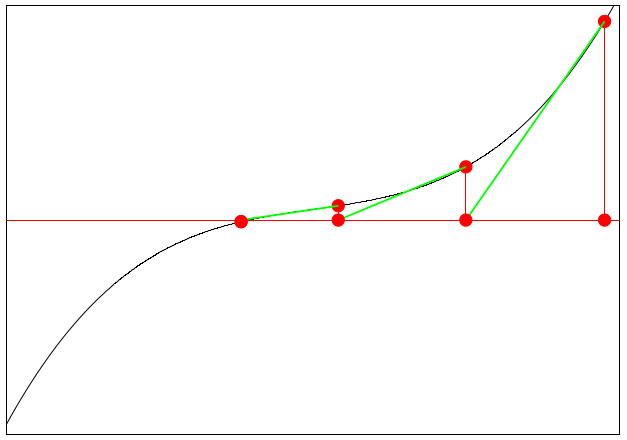
\includegraphics[width=7cm]{img/roots15.png}
	\end{figure}
	
	Applicando il metodo di Newton-Raphson si ottiene la seguente sequenza:
	
	\begin{center}
		\begin{tabular}{c c c}
			\hline
			$i$ & $x_r$ & $f(x_r)$ \\
			\hline
			0 & 1.9    &  \\
			1 & 1.1173 & 0.60 \\
			2 & 0.4825 & 0.22 \\
			4 & -0.4714 & 0.02 \\
			5 & -0.4257 & 0.0006 \\
			7 & -0.4239 & < $10^{-8}$ \\
			\hline
		\end{tabular}
	\end{center}

\end{multicols}

Si osserva una convergenza molto più rapida rispetto al metodo di bisezione.

\subsection{Analisi dell'errore}

Per comprendere meglio la velocità di convergenza, consideriamo una radice \( x_r \) e poniamo $x = x_r + \epsilon$ , così che sviluppando la funzione:

\[
f(x + \epsilon)\ =\ f(x)\, +\, \epsilon\, f'(x)\, +\, \frac{\epsilon^2}{2}\, f''(x)\ \ .
\]

Stavolta non buttiamo via il termine del secondo ordine così applicando l'iterazione di Newton-Raphson di eq.(\ref{Newton-Raphson}) si ottiene una stima per l'errore:

\[
\epsilon_{i+1} = - \frac{\epsilon_i^2 f''(x_i)}{2 f'(x_i)}.
\]

Questo mostra che l'errore si riduce \textbf{quadraticamente}, ovvero

\[
\epsilon_{i+1} \sim \epsilon_i^2,
\]

il che spiega la rapidissima convergenza del metodo.

\subsection{Osservazioni sul metodo di Newton-Raphson}

Il metodo di Newton-Raphson presenta numerosi vantaggi:

\begin{multicols}{2}
\begin{itemize}
	\item convergenza molto rapida;
	\item esatto per funzioni lineari;
	\item estendibile a più dimensioni;
	\item non richiede il bracketing della radice.
\end{itemize}
\end{multicols}

Tuttavia presenta anche alcune criticità:

\begin{multicols}{2}
\begin{itemize}
	\item richiede una buona stima iniziale, altrimenti...
	\item ... può divergere o oscillare;
	\item può bloccarsi in punti stazionari;
	\item fallisce in presenza di discontinuità;
	\item richiede che \( f'(x) \neq 0 \).
\end{itemize}
\end{multicols}
	
	
\begin{figure}[H]
		\centering
		\label{newton cotes comments}
		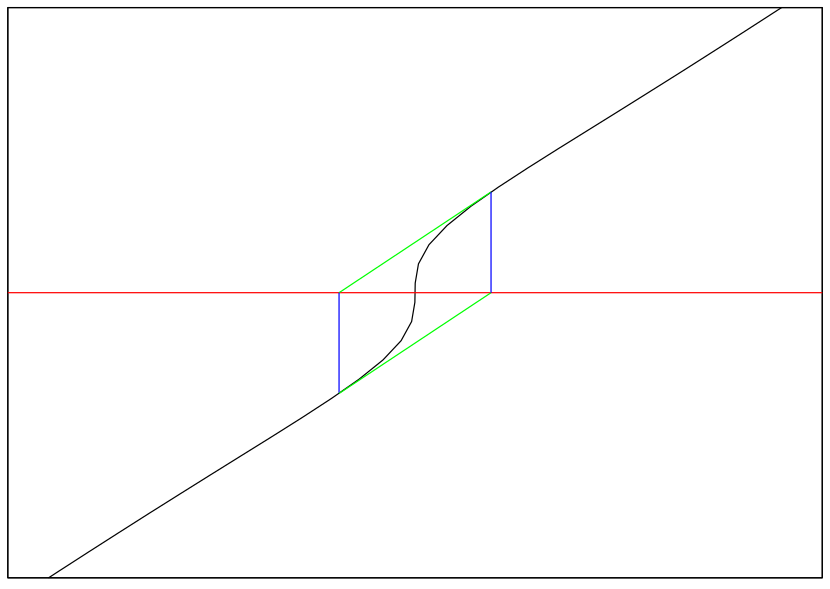
\includegraphics[width=6cm]{img/roots16.png}
		\caption{esempio visivo di radice che fa andare in palla il metodo di Newton-Raphson.}
\end{figure}



%
%
%
\section{Caso dei polinomi, metodo di Laguerre}

Nel caso particolare dei polinomi esistono metodi specifici molto efficienti.

Consideriamo un polinomio scritto nella sua forma fattorizzata:

\[
P_n(x)\ =\ (x - x_1)\, (x - x_2)\, \cdots\, ( x - x_n).
\]

Si può portare il prodotto ad essere una sommatoria usando il logaritmo:

\[
\ln |P_n(x)|\ =\ \sum_i\, \ln |x - x_i|.
\]

Derivando:

\[
\frac{d}{dx} \ln |P_n(x)|\ =\ \sum_i\, \frac{1}{x - x_i}\
=\ \frac{P'_n(x)}{P_n(x)}\ \equiv\ G,
\]

Questa nuova quantità $G$ possiamo trattarla come una grandezza che ci dice in base al punto $x$ in cui siamo quanto siamo vicini a ciascuna radice (vedi l'inverso, se siamo molto vicini, $G$ diventa molto grande). In particolare la radice più vicina $x_k$ contribuirà molto di più nella sommatoria, quindi $x_k\approx x - \frac{1}{G}$ in prima approssimazione.

\[
\frac{d^2}{dx^2} \ln |P_n(x)|\ =\
\sum_i\, \frac{1}{(x - x_i)^2}
\ =\ \left[\frac{P'_n}{P_n}\right]^2\, -\, \frac{P''_n}{P_n}\ =\ H.
\]

Possiamo esprimere H in funzione del polinomio e di G, che porta informazioni sulla distanza delle radici: $H=G^2 - P_n ''/P_n$  .

Si ottiene quindi $G\,=\, \frac{1}{a} + \frac{n-1}{b}$ e $H\,=\, \frac{1}{a^2} + \frac{n-1}{b^2}$, dove in particolare $a$ è la distanza della radice più vicina ($a=x-x_k$) e $b$ è la distanza di 'tutte' le altre radici (facendo finta siano tutte ugualmente distanti, $\sum_{i\neq k} (x - x_i)^{-2}\approx\frac{n-1}{b}$), così abbiamo una prima stima infine della distanza della radice:

\[
a = \frac{n}{G \pm \sqrt{(n-1)(nH - G^2)}}.
\]

Il metodo consiste nell'iterare $x \rightarrow x - a$ , scegliendo il segno che massimizza il denominatore.

%
%
%
\vspace{0.5cm}
\section{Generalizzazione a più dimensioni di Newton-Raphson}

Il problema della ricerca degli zeri si estende naturalmente a più dimensioni.

Si considerano sistemi del tipo $f_i(\mathbf{X}) = 0$, con $i=1,\dots , n$, dove \( \mathbf{X}=(x_1,\, \dots ,\, x_n) \) è un vettore in \( \mathbb{R}^n \).

Si generalizza il metodo di Newton-Raphson scrivendo

\[
f_i(\mathbf{X} + \delta)\ \approx\ f_i(\mathbf{X})\, +\, \sum_j\, \frac{\partial f_i}{\partial x_j}\, \delta_j.
\]

Definendo $a_{ij} = \frac{\partial f_i}{\partial x_j}$, coefficienti dello jacobiano, si ottiene il sistema lineare:

\[
\sum_j\, a_{ij}\, \delta_j\ =\ -f_i(\mathbf{X}).
\]

Risolvendo per \( \delta \) si ottiene  $\delta_j = - \sum_i (a_{ij})^{-1} f_i(\mathbf{X})$  e si itera seguendo  $X_i^{(\text{new})} = X_i^{(\text{old})} + \delta_i$  .

\begin{multicols}{2}
\paragraph{Esempio bidimensionale: }

Un esempio di sistema non lineare è

\[
f_1(x,y) = x^2 + y^2 - 1,
\]

\[
f_2(x,y) = y - x^2 + \frac{x}{2}.
\]

La soluzione corrisponde all'intersezione delle due curve.

\begin{figure}[H]
	\centering
	\label{esempio bidi}
	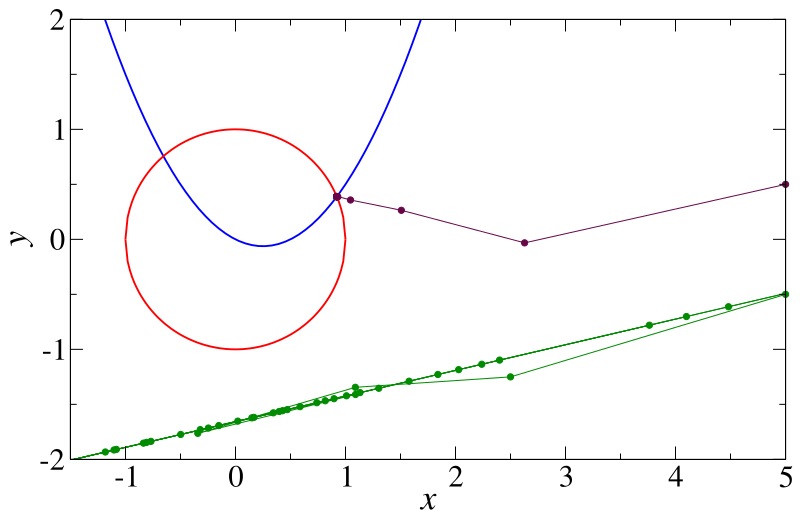
\includegraphics[width=6cm]{img/roots18.png}
	\caption{esempio bidimensionale}
\end{figure}

\end{multicols}

\section{Conclusioni}

Riassumendo:

\begin{itemize}
	\item è sempre necessario avere un'idea preliminare della posizione della radice;
	\item il metodo di bisezione è robusto ma lento;
	\item il metodo di Newton è rapido ma delicato;
	\item per i polinomi esistono metodi dedicati;
	\item in più dimensioni il metodo di Newton è lo strumento principale, ma è sensibile alle condizioni iniziali.
\end{itemize}

\bigskip

La scelta del metodo più adatto dipende quindi dal problema specifico, dal grado di informazione disponibile sulla funzione e dal compromesso desiderato tra stabilità e velocità di convergenza.
	
	\newpage
	
	\chapter{Introduzione all'analisi numerica nell'integrazione}

Il problema dell'integrazione numerica può essere risolto, in linea di principio, con l'aiuto di equazioni differenziali ordinarie (\underline{ODEs}):
\[ \int^x_a\, f(y)\, dy\ =\ g(x) \quad \quad \Rightarrow \quad \quad \frac{d\, g}{d\, x}\ =\ f(x)\ , \]
con boundary $x_0=a$.

Sebbene questa osservazione sia formalmente corretta, è preferibile sviluppare metodi diretti di integrazione numerica, analogamente a quanto si è fatto per le equazioni differenziali, dove la scelta del metodo appropriato non è affatto immediata.

Un algoritmo generale di integrazione numerica ha la struttura

\[
\int_a^b f(x)\,dx = \sum_i w_i f(x_i),
\]

dove $w_i$ sono pesi e $x_i$ i nodi di valutazione. 

In genere si pone $x_i = a + i h$ con passo $h$ uniforme e si scrive $f_i = f(x_i)$.

\begin{multicols}{2}	
	Si distinguono due grandi classi di formule:
	
	\begin{itemize}
		\item \textbf{Formule chiuse}: utilizzano anche i valori agli estremi $a$ e $b$.
		\item \textbf{Formule aperte}: non utilizzano uno o entrambi gli estremi.
	\end{itemize}
	
	Il vantaggio principale delle formule aperte è che possono essere utilizzate quando la funzione non è definita agli estremi, pur essendo l'integrale ben definito.
	
	\begin{figure}[H]
		\centering
		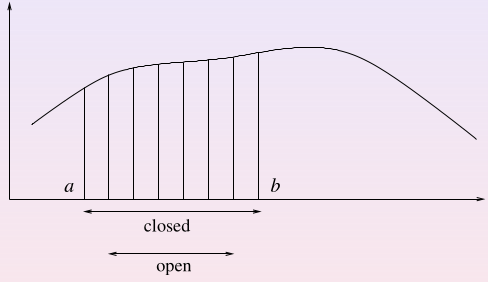
\includegraphics[width=\linewidth]{img/integration_1.png}
		\caption{differenza fra intervalli presi in considerazione da classi di formule chiuse e aperte}
	\end{figure}
\end{multicols}



\subsection{Formule di Newton–Cotes su intervallo singolo}

Le formule di Newton-Cotes nascono dalla divisione in intervalli equispaziati e dalla successiva integrazione esatta di un polinomio che passa per quegli $n$ punti (interpolazione).

La regola fondamentale dell'integrazione numerica, la formula di Newton-Cotes di grado più basso è la \underline{regola dei trapezi}, che usa una retta tesa fra due punti successivi per interpolare:

\begin{equation}
	\label{trapezoidal-rule}
	\int_{x_1}^{x_2}\, f(x)\, dx\ =\
	\frac{1}{2}\, h \, [f_1 + f_2] + \mathcal{O}(h^3\, f^{''})\ ,\
\end{equation}  

questa è esatta per funzioni lineari, ad esempio $f(x)=x$. 

Si ottiene interpolando $f(x)$ con il polinomio lineare che passa per i punti $(x_1,\, f_1)$ e $(x_2,\, f_2)$:

\[ f(x)\ =\ f_1\, +\, (f_2\, -\, f_1)\, x\ \ , \]

e in seguito integrando sull'intervallo normalizzato $0 \le x \le 1$.

Formule di ordine superiore si ottengono interpolando con polinomi di grado più elevato. Ad esempio,

\begin{equation}\label{Simpson's rule}
	\int_{x_1}^{x_3}\, f(x)\, dx\ =\ h\, \left[
	\frac{1}{3}\, f_1\, +\, \frac{4}{3}\, f_2\, +\, \frac{1}{3}\, f_3\right]\, +\,	\mathcal{O}(h^5\, f^{(4)})\ \ ,
\end{equation} 

che è la \underline{regola di Simpson}, esatta per polinomi fino al terzo grado.
La regola di Simpson nasce dall'interpolazione con una parabola $P(x)=Ax^x + Bx+C$ su tre punti equispaziati $x_0$, $x_1$, $x_2$ con funzione da integrare $f_0=f(x_0)$, $f_1$, $f_2$. Facciamo un cambio di variabile $t=x-x_i$ così che i tre punti diventino $t=0,\, h,\, 2h$, riscrivendo la parabola come $P(t)=at^2+bt+c$. Si va ora ad imporre che $P(t=0)=c=f_0$, mentre nel secondo punto $P(t=h)=ah^2+b^h+c=f_1$ e nel terzo $P(t=2h)=4ah^2+2bh+c=f_2$. Invertendo questo sistema di equazioni si trova che $c=f_0$, $a=\frac{f_2-2f_1+f_0}{2h^2}$ mentre $b=\frac{f_1-f_0}{h}-ah$.
A questo punto l'integrale $\int_{x_0}^{x_2} f(x) dx\approx \int_0^{2h} P(t) dt= \int_0^{2h} at^2+bt+f_0 dt$ è facilmente sostituibile con le dovute sostituzioni di $a$ e $b$ nelle forme appena trovate e con una semplice integrazione del polinomio si ottiene proprio Simpson: $\int_{x_0}^{x_2} f(x) dx\approx \frac{h}{3} [f_0 + 4\,f_1 + f_2]$.

Analogamente, per cinque punti la formula di Newton-Cotes diventa:

\[ \int_{x_1}^{x_5}\, f(x)\, dx\ =\ h\, \left[ \frac{14}{45}\, f_1\, +\, \frac{64}{45}\, f_2\, +\, \frac{24}{45}\, f_3\, +\, \frac{64}{45}\, f_4\, +\, \frac{14}{45}\, f_5\, \right]\, +\, \mathcal{O}(h^7\, f^{(6)})\ \ .\]

\subsection{Alcune formule locali}

È utile osservare anche relazioni locali su intervalli elementari:

\[ \int_{x_0}^{x_1}\, f(x)\, dx\ =\ h[f_1]\, +\, \mathcal{O}(h^2\, f')\ \ ,\]


\[ \int_{x_0}^{x_1}\, f(x)\, dx\ =\ h\, \left[ \frac{3}{2}f_1\, -\, \frac{1}{2}f_2 \right]\, +\, \mathcal{O}(h^3\, f'')\ \ .\]

La prima è un semplice rettangolo, una Newton-Cotes aperta di ordine 0 con errore di ordine $h^2$, mentre la seconda formula è una Newton-Cotes aperta di ordine 1 e si ottiene interpolando linearmente $f(x)\ =\ f_1 + x\, (f_2 - f_1)$, e integrando nell'intervallo $-1 \le x \le 0$:

\[ \int_{-1}^{0} f(x)\,dx\ =\ -(-f_1)\, -\, \frac{(-1)^2}{2}\, (f_2 - f_1) \ =\ \left[ \frac{3}{2}f_1 - \frac{1}{2}f_2\right]\ .\]

Formule di ordine superiore si ottengono usando approssimazioni polinomiali di grado crescente.

\subsection{Intervalli estesi}

Passando a intervalli estesi, dalla regola dei trapezi in eq.(\ref{trapezoidal-rule}) segue una regola dei trapezi estesa:

\begin{equation} \label{regola-dei-trapezi-estesa}
	\int_{x_1}^{x_n} f(x)\,dx\ =\ h\, \left[
	\frac{1}{2}f_1\, +\, f_2\, +\, f_3\, +\, \dots\, +\, \frac{1}{2}f_n
	\right]\, +\,
	\mathcal{O}\!\left(\frac{(x_n-x_1)^3}{N^2}\, f''\right)\ \ ,
\end{equation} 

dove $N$ è il numero di suddivisioni.

Dalla regola di Simpson in eq.(\ref{Simpson's rule}), si ottiene invece:

\begin{equation}\label{Simpson-esteso}
	\int_{x_1}^{x_n}\, f(x)\,dx\ =\ h\, \left[ \frac{1}{3}f_1\,+\,\frac{4}{3}f_2\,+\,\frac{2}{3}f_3\,+\,\frac{4}{3}f_4\,\dots\,+\,\frac{4}{3}f_{n-1}\,+\,\frac{1}{3}f_n\right]
	\,+\,\mathcal{O}\!\left(\frac{1}{N^4}\right)\ \ .
\end{equation} 

Di seguito un'implementazione in C della regola dei trapezi e di Simpson:
\lstinputlisting[style=Cstyle,
	caption={Implementazione del metodo dei trapezi},
	label={lst:trapezi}]{trapezi.c}

Si può combinare una formula aperta locale (singolo intervallo) con una formula chiusa estesa di quelle appena scritte per ottenere una formula aperta su intervallo esteso. 

Ad esempio, combinando

\[
\int_{x_0}^{x_1} f(x)\,dx
=
h f_1 + \mathcal{O}(h^2 f')
\]

con la regola dei trapezi estesa su $[x_1,x_n]$ vista in eq.\ref{regola-dei-trapezi-estesa}, si ottiene:

\[ \int_{x_0}^{x_n}\, f(x)\, dx\ =\ h\, \left[ \frac{3}{2}f_1\, +\, f_2\, +\, f_3\, +\, \dots\, +\, \frac{3}{2}f_{n-1}\right]\,+\, \mathcal{O}\!\left(\frac{1}{N^2}\right)\ \ .\]

Analogamente, combinando la formula aperta di ordine superiore

\[ \int_{x_0}^{x_1} f(x)\,dx \ =\ h\,\left[ \frac{23}{12}f_1\,-\,\frac{16}{12}f_2\,+\,\frac{5}{12}f_3\right]\, +\, \mathcal{O}(h^4 f^{(3)})\ \ , \]

con la regola di Simpson estesa eq.(\ref{Simpson-esteso}), si ottiene una formula complessiva di ordine $\mathcal{O}(1/N^4)$.

\[ \int_{x_0}^{x_n}\, f(x)\, dx\ =\ h\, \left[ \frac{27}{12}f_1\, +\, 0\, +\, \frac{13}{12}f_3\, +\, \frac{4}{3} f_4\, +\,  \dots\, +\, \frac{4}{3}f_{n-4}, +\, \frac{13}{12}f_{n-3}\, +\, 0\, +\, \frac{27}{12}f_{n-1}\right]\,+\, \mathcal{O}\!\left(\frac{1}{N^2}\right)\ \ .\]

\bigskip

Il problema pratico fondamentale rimane: quanti passi bisogna utilizzare?

Se si usa la regola dei trapezi come blocco base, l'errore scala come $boxed{\frac{K}{N^2}}$, raddoppiando $N$, l'errore si riduce di un fattore 4. Questo comportamento è alla base dei metodi di raffinamento successivi.

\subsection{Valutazione dell’errore e formula esatta dei trapezi}

L'errore può essere valutato facendo la differenza fra l'integrale calcolato con N steps e quello calcolato con 2N steps.

Per stimare in modo più preciso l’errore della regola dei trapezi estesa, si può utilizzare la sua espressione esatta in termini dei numeri di Bernoulli:

\[
\int_{x_1}^{x_n} f(x)\,dx
\ =\
h\ \left[
\frac{1}{2}f_1\, +\, f_2\, +\, \dots\, +\, \frac{1}{2}f_n
\right]
\,-\,
\frac{B_2 h^2}{2!}\left(f'_n - f'_1\right)
\,-\,
\frac{B_{2k} h^{2k}}{(2k)!}\,
\left(f^{(2k-1)}_n\, -\, f^{(2k-1)}_1\right)
\,-\, \dots
\]

dove $B_k$ sono i numeri di Bernoulli, definiti tramite

\[
\frac{t}{e^t - 1}
\ =\
\sum_{n=0}^{\infty}\, B_n\, \frac{t^n}{n!}.
\]

Il termine dominante dell’errore è proporzionale a $h^2$, cioè a $1/N^2$. Se indichiamo con $S_N$ l’integrale calcolato con $N$ suddivisioni e con $S_{2N}$ quello con $2N$, possiamo eliminare il termine in $h^2$ combinando linearmente i due risultati:

\[
S = \frac{4}{3} S_{2N} - \frac{1}{3} S_N.
\]

In questo modo l’errore dominante diventa dell’ordine $h^4$.

\subsection{Integrazione di Romberg}

L’idea precedente può essere iterata. Se una combinazione elimina il termine in $h^2$, si può ripetere il procedimento per eliminare anche il termine in $h^4$, poi quello in $h^6$, e così via.

Il metodo di Romberg consiste nel:

\begin{itemize}
	\item calcolare l’integrale con una sequenza di suddivisioni $N, 2N, 4N, \dots$;
	\item costruire combinazioni lineari che eliminano progressivamente i termini dominanti dell’errore;
	\item interpretare il risultato come un’estrapolazione razionale nel limite $N \to \infty$.
\end{itemize}

Il metodo produce una tabella triangolare di approssimazioni con ordine crescente di accuratezza.

Di seguito un'implementazione in C dell'integrazione di Romberg presa dal \emph{Numerical Recipes in C: The art of scientific programming}:

\lstinputlisting[style=Cstyle,
				caption={Implementazione del metodo di Romberg},
				label={lst:romberg}]{Romberg.c}


\subsection{Quadrature Gaussiane}
Vogliamo approssimare integrali del tipo

\[\int W(x) f(x)\, dx\ =\ \sum_{j=1}^{N} w_j f(x_j)\ \ ,\]

dove: $W(x) > 0$ è una funzione peso, $\int W(x)\,dx = 1$ (normalizzazione) ed i nodi $x_j$ non sono necessariamente equispaziati.

Introduciamo il prodotto scalare pesato

\[\langle f\, |\, g \rangle\ =\ \int\, W(x)\, f(x)\, g(x)\, dx\ \ .\]

Si definisce una successione di polinomi ortogonali $\{p_k(x)\}$ tramite la ricorrenza a tre termini:

\[ p_{-1}(x)=0, \qquad p_0(x)=1\ \ ,\]

\[ p_{j+1}(x)\ =\ (x-a_j)\, p_j(x) - b_j\, p_{j-1}(x)\ \ ,\]

con coefficienti:

\[a_j = \frac{\langle x\, p_j\, |\, p_j \rangle}{\langle p_j\, |\, p_j \rangle},
\qquad
b_j =\frac{\langle p_j\, |\, p_j \rangle}{\langle p_{j-1}\, |\, p_{j-1} \rangle}\ \ .
\]

Proprietà fondamentali:

\begin{itemize}
	\item $p_j$ è monico e di grado $j$,
	\item $p_j$ possiede $j$ zeri reali semplici,
	\item gli zeri sono interlacciati con quelli di $p_{j-1}$.
\end{itemize}

Assumiamo che $f(x)$ sia un polinomio di grado al massimo $2N-1$. Può essere scritto in generale come $f(x)\,=\, p_N(x)q_f(x)\,+\, r_f(x)$ con $q_f(x)$ e $r_f(x)$ polinomi di grado $<N$. In particolare:

\[ q_f(x)=\sum_{N-1} a_k p_k (x)\ , \qquad a_k=\frac{\langle p_k|q_f\rangle}{\langle p_k |p_k\rangle}\ \ ,\]

\[ r_f(x)=\sum_{N-1} b_k p_k (x)\ , \qquad b_k=\frac{\langle p_k|r_f\rangle}{\langle p_k |p_k\rangle}\ \ ,\]

Vale che:

\[ \int W(x)\,f(x)\,dx\ =\ \int W(x)\, (P_N(x)q_f(x) + r_f(x))\, dx\ =\ \sum w_j\, (P_N(x)q_f(x) + r_f(x))\ \ , \]

che, \underline{nel caso in cui le $x_j$ siano radici di $p_N$}, diventa:

\[ \int W(x)\,f(x)\,dx\ =\  \sum\, w_j(x)\, r_f(x_j) \ =\ \int W(x)\, r_f(x)\, dx\ \ , \]

Ma per ipotesi, $r_f$ era di un grado in meno rispetto ad N, quindi l'integrale qui sopra è esatto.

Sappiamo che le $x_j$ sono radici di $p_n$, cosa dire per le $w_j$?  

Grazie all'ortogonalità si ottiene il sistema lineare:

\[ \begin{pmatrix}
	p_0(x_1) & p_0(x_2) & \dots & p_0(x_N) \\
	p_1(x_1) & p_1(x_2) & \dots & p_1(x_N) \\
	\vdots   & \vdots   &       & \vdots   \\
	p_{N-1}(x_1) & p_{N-1}(x_2) & \dots & p_{N-1}(x_N)
\end{pmatrix}\
\begin{pmatrix}
	w_1 \\ w_2 \\ \vdots \\ w_N
\end{pmatrix}
\ =\
\begin{pmatrix}
	\int W(x)p_0(x)\,dx \\
	0 \\
	\vdots \\
	0
\end{pmatrix}\ \ .\]

Se scegliamo $x_j$ come zeri di $p_N(x)$, il sistema è ben posto e la formula risulta esatta fino al grado $2N-1$.

I pesi si possono esprimere direttamente come:

\[
w_j
=
\frac{\langle p_{N-1}|p_{N-1}\rangle}
{p_{N-1}(x_j)\, p'_N(x_j)}.
\]


\begin{center}
	\begin{tabular}{|l|l|c|c|}
		\hline
		Intervallo & $W(x)$ & "\emph{Recurrence}" & Nome \\
		\hline
		$(-1,1)$ & $1$ & $(i+1)P_{i+1}\,=\,(2i+1)xP_i\, +\, iP_{i-1}$ & \textbf{Legendre} \\
		$(-1,1)$ & $\displaystyle\frac{1}{\sqrt{1-x^2}}$ & $T_{i+1}\, =\, 2xT_i\,- \,T_{i-1}$ & \textbf{Chebyshev} \\
		$(0,\infty)$ & $x^c e^{-x}$ & $\begin{aligned} (i+1)L^c_{i+1}\,=\, (-x+2i+c+1) L^c_i \\ -(i+c)L^c_{i-1}\ \ c=0,1,\dots \end{aligned}$ &\textbf{Laguerre} \\
		$(-\infty,\infty)$ & $e^{-x^2}$ & $H_{i+1}\,=\, 2xH_i\,-\,2iH_{i-1}$ &\textbf{Hermite} \\
		\hline
	\end{tabular}
\end{center}

\subsubsection{Tabella Gauss–Legendre}

Per $W(x)=1$ su $(-1,1)$:

\begin{center}
	\begin{tabular}{|c|c|c|}
		\hline
		$n$ & $x_j$ & $w_j$ \\
		\hline
		2 & $\pm 0.577350269189626$ & $1.0$ \\
		\hline
		3 & $\pm 0.774596669241483$ & $0.555555555555556$ \\
		& $0$ & $0.888888888888889$ \\
		\hline
		4 & $\pm 0.861136311594053$ & $0.347854645137454$ \\
		& $\pm 0.339981043584856$ & $0.652145154862546$ \\
		\hline
	\end{tabular}
\end{center}

Per integrare su $(a,b)$ mappiamo l'intervallo in (-1,1), grazie al cambio di variabile:

\[
y = \frac{2(x-a)}{b-a} - 1 \ \ ,
\qquad
x = a + \frac{(y+1)(b-a)}{2}\ \ .
\]

Allora si ottiene:

\[
\int_a^b\, f(x)\,dx
\ =\
\frac{b-a}{2}
\int_{-1}^{1}
f\! \,\left(a + \frac{(y+1)(b-a)}{2}\right) dy.
\]

\subsection{Integrali impropri}

Un integrale è \underline{improprio} se:

\begin{itemize}
	\item uno dei limiti è infinito,
	\item la funzione diverge in un estremo ma è integrabile,
	\item è presente una singolarità interna.
\end{itemize}

\subsubsection{Limiti infiniti}

Trattando un integrale improprio con limiti infiniti (che può voler dire anche solo molto molto grandi), per $ab>0$ si può fare un cambio di variabile del tipo:

\[ \int_a^b f(x)\,dx
\ =\
\int_{1/a}^{1/b}
\,\frac{1}{t^2} \,f\!\left(\frac{1}{t}\right) \,dt\ \ ,\]

Chiaro che un cambio di variabile del genere significa che rimaniamo a debita distanza dal punto $x=0$. Se $ab<0$, si divide l’integrale in due parti in modo che l'integrale che contiene lo zero non sia trasformato.

\subsubsection{Singolarità integrabile all’estremo}

Supponiamo che l'integrale abbia una singolarità integrabile di tipo \emph{power law}:

\[
f(x) \sim (x-a)^{-\gamma}\ ,
\qquad 0 \le \gamma < 1\ \ ,
\]

si usa la mappatura $t = (x-a)^{1-\gamma}$ così che si ottenga:

\[
\int_a^b\, f(x)\,dx
\ =\
\frac{1}{1-\gamma}
\,\int_0^{(b-a)^{1-\gamma}}
t^{\frac{\gamma}{1-\gamma}}\, 
f\!\left(t^{\frac{1}{1-\gamma}}\, +\, a\right) \,dt\ \ ,
\]

con $b>a$. Similmente se la singolarità è in b:

\[
\int_a^b\, f(x)\,dx
\ =\
\frac{1}{1-\gamma}
\,\int_0^{(b-a)^{1-\gamma}}
t^{\frac{\gamma}{1-\gamma}}\, 
f\!\left( b\, -\, t^{\frac{1}{1-\gamma}}\right) \,dt\ \ ,
\]

Alternativamente un metodo più banale ma più situazionale è aggiungere e sottrarre una funzione con stessa singolarità di cui si conosce l'integrale.

\subsubsection{Singolarità interna}

Se la divergenza è in un punto interno $x=y$ vi sono due casi:

\begin{itemize}
	\item L'integrando è tale che la divergenza è integrabile su $(a,y)$ e $(y,b)$. In tal caso si divide l’intervallo e si utilizza la prescrizione per integrale improprio con limite infinito;
	\item Se l’integrale esiste solo come valore principale, si riorganizza l’integrando per ottenere cancellazione numerica.
\end{itemize}

\subsubsection{Singolarità di tipo Cauchy}

Un integrale che andiamo spesso a risolvere in fisica è nella forma:

\[ I(y)\ =\ \mathrm{P}\,\int_a^b\, \frac{f(x)}{x-y}\, dx\ \ ,\]

Uno dei modi di risolvere quest'integrale, che assume che $f(x)$ sia continua nella sua derivata prima e seconda, usa l'integrazione per parti:

\[ I(y)\ =\
\left[\ln|x-y|\,f(x)\right]\,_a^b\,
-\,
\int_a^b\, \ln|x-y|\,f'(x)\,dx\ \ .
\]

Se necessario, si integra nuovamente:

\[\begin{aligned}
	I(y)\ =\
	&\left[\ln|x-y|\,f(x)\right]_a^b
	\, -\,
	\left[(x-y)\ln|x-y|-(x-y)\right]f'(x)\Big|_a^b
	\, +\, \dots\\
	&\dots \, +\, \int_a^b [(x-y)\ln|x-y|-(x-y)] f''(x)\,dx\ \ .
\end{aligned}\]

Ora l'integrando finale è regolare salvo discontinuità di $f''$.

\subsubsection{Formule aperte}

Una formula aperta utile è:

\[\begin{aligned}
	\int_{x_1}^{x_n} f(x)\,dx
	\ =\ 
	&h\left[
	f_{3/2}+f_{5/2}+\dots+f_{n-1/2}
	\right]
	\, +\, \dots\\
	&\dots \, +\, \sum_{k=1}^{\infty}
	\frac{B_{2k} h^{2k}}{(2k)!}
	\left(1-2^{-2k+1}\right)
	\left(f^{(2k-1)}_n - f^{(2k-1)}_1\right)\ \ .\end{aligned}
\]

Qui i $B_{2k}$ sono numeri di Bernoulli.

In questo caso la semplice riduzione del passo non permette il riuso diretto dei punti precedenti; tuttavia triplicando la suddivisione si possono costruire procedure di raffinamento analoghe a Romberg.
	
	\newpage
	
	\input{ODE.tex}
	
	\newpage
	\appendix

	%\emph{ Tutte le appendici di seguito non provengono dal corso ``Metodi numerici per la fisica'' (``Computational physics laboratory''), ma dal corso del master in ingegneria nucleare ``Physics and numerical models for nuclear reactors'', del prof. Valerio Giusti. }

\chapter{Metodo delle differenze finite}

\subsection*{Introduzione}

Il metodo delle differenze finite è una tecnica numerica utilizzata per approssimare le derivate di una funzione mediante valori della stessa in punti discreti.

Conosciamo bene la definizione di derivata come rapporto incrementale, possiamo quindi usare punti discreti della funzione per svolgere questo rapporto ed approssimare la funzione:

\[
\frac{d\varphi}{dx} =
\lim_{h \to 0}
\frac{\varphi(x+h)-\varphi(x)}{h}
\qquad \text{rapporto incrementale in avanti}
\]

\[
\frac{d\varphi}{dx} =
\lim_{h \to 0}
\frac{\varphi(x)-\varphi(x-h)}{h}
\qquad \text{rapporto incrementale all\'indietro}
\]

\[
\frac{d\varphi}{dx} =
\lim_{h \to 0}
\frac{\varphi(x+h)-\varphi(x-h)}{2\,h}
\qquad \text{rapporto incrementale centrato}
\]

Questo metodo ci dice che considerando il dominio $x\in [0,X]$ e ponendo la \emph{mesh} di N punti, tale che l'intervallo sia $h=X/N$, l'approssimazione della derivata calcolata con punti discreti della funzione può essere calcolata con:

\begin{equation}
	\frac{ d\varphi }{ dx }|_i\,\approx\, \frac{ \varphi_{i+1}-\varphi_i }{h}\ ,\quad 
	\frac{ d\varphi }{ dx }|_i\,\approx\, \frac{ \varphi_{i}-\varphi_{i-1} }{h}\ ,\quad 
	\frac{ d\varphi }{ dx }|_i\,\approx\, \frac{ \varphi_{i+1}-\varphi_{i-1} }{2\,h}\ \ .
\end{equation}

\begin{multicols}{2}
	Nessuna di queste formule è migliore delle altre in ogni occasione, per ogni funzione che si voglia derivare.
	
	Nel caso in figura si vede come il rapporto in avanti è qui il migliore per approssimare la derivata prima.
	
	
	\begin{figure}[H]
		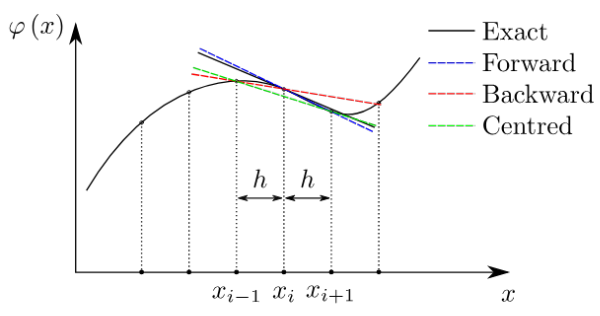
\includegraphics[width=7cm]{img/finitedifferences.png}
		\caption{Prova di applicazione del metodo delle differenze finite al calcolo della derivata prima di una generica funzione polinomiale.}
	\end{figure}
	
\end{multicols}


\subsection*{Accuratezza delle approssimazioni}

Per studiare l'errore utilizziamo lo sviluppo di Taylor.

\[
\varphi(x) =
\varphi(x_0)
+
(x-x_0)\left.\frac{d\varphi}{dx}\right|_{x_0}
+
\frac{(x-x_0)^2}{2}
\left.\frac{d^2\varphi}{dx^2}\right|_{x_0}
+
\frac{(x-x_0)^3}{6}
\left.\frac{d^3\varphi}{dx^3}\right|_{x_0}
+ \dots
\]

Ponendo $x_i = x_0$ otteniamo per $\varphi_{i+1}\,,\ \varphi_{i-1}$:

\[
\varphi_{i+1} =
\varphi_i
+
(x_{i+1}-x_i)
\left.\frac{d\varphi}{dx}\right|_i
+
\frac{(x_{i+1}-x_i)^2}{2}
\left.\frac{d^2\varphi}{dx^2}\right|_i
+
\frac{(x_{i+1}-x_i)^3}{6}
\left.\frac{d^3\varphi}{dx^3}\right|_i
+ \dots
\]

\[
\varphi_{i-1} =
\varphi_i
+
(x_{i-1}-x_i)
\left.\frac{d\varphi}{dx}\right|_i
+
\frac{(x_{i-1}-x_i)^2}{2}
\left.\frac{d^2\varphi}{dx^2}\right|_i
+
\frac{(x_{i-1}-x_i)^3}{6}
\left.\frac{d^3\varphi}{dx^3}\right|_i
+ \dots
\]

Poiché $x_{i+1}-x_i = h$, si ottiene

\begin{equation}\label{i+1 e i-1}
	\begin{aligned}
	\varphi_{i+1} &=
	\varphi_i +
	h \left.\frac{d\varphi}{dx}\right|_i +
	\frac{h^2}{2}\left.\frac{d^2\varphi}{dx^2}\right|_i +
	\frac{h^3}{6}\left.\frac{d^3\varphi}{dx^3}\right|_i + \dots \\
	\varphi_{i-1} &=
	\varphi_i -
	h \left.\frac{d\varphi}{dx}\right|_i +
	\frac{h^2}{2}\left.\frac{d^2\varphi}{dx^2}\right|_i -
	\frac{h^3}{6}\left.\frac{d^3\varphi}{dx^3}\right|_i
	+ \dots
	\end{aligned}
\end{equation}

Da queste espansioni in eq.(\ref{i+1 e i-1}) possiamo riottenere la derivata con metodo forward e backward:

\begin{equation}\label{der}
	\begin{aligned}
	\left.\frac{d\varphi}{dx}\right|_i &=
	\frac{\varphi_{i+1}-\varphi_i}{h} -
	\frac{h}{2}\left.\frac{d^2\varphi}{dx^2}\right|_i -
	\frac{h^2}{6}\left.\frac{d^3\varphi}{dx^3}\right|_i
	+ \dots\ =\\
	& =
	\frac{\varphi_{i+1}-\varphi_i}{h}
	+ O(h)\qquad \text{(\textbf{forward})}\\
	\left.\frac{d\varphi}{dx}\right|_i &=
	\frac{\varphi_i-\varphi_{i-1}}{h}
	\, +\,
	\frac{h}{2}\left.\frac{d^2\varphi}{dx^2}\right|_i
	\, -\,
	\frac{h^2}{6}\left.\frac{d^3\varphi}{dx^3}\right|_i
	+ \dots\ =\\
	& =\ \frac{\varphi_i-\varphi_{i-1}}{h}\, +\, O(h)
	\qquad \text{(\textbf{backward})}
	\end{aligned}	
\end{equation}

Sommando le due espressioni in eq.(\ref{der}) si ottiene

\[
\left.\frac{d\varphi}{dx}\right|_i
\ =\
\frac{\varphi_{i+1}-\varphi_{i-1}}{2h}\,
-\,
\frac{h^2}{6}\,
\left.\frac{d^3\varphi}{dx^3}\right|_i
\,+\,  \dots\ =\
\frac{\varphi_{i+1}-\varphi_{i-1}}{2h}
\,+\,
O(h^2)
\]

Questa formula ha un errore di ordine $h^2$, quindi è più accurata rispetto alle approssimazioni forward e backward che hanno errore $O(h)$.


\subsection*{Approssimazione della derivata seconda}

Sottraendo le due espansioni in eq.(\ref{der}) si ottiene

\[
0\ =\
\frac{\varphi_{i+1}-\varphi_i}{h}
\,-\,
\frac{\varphi_i-\varphi_{i-1}}{h}
\,-\,
h
\left.\frac{d^2\varphi}{dx^2}\right|_i
\,+\,
O(h^3)
\]

da cui segue la formula standard della derivata seconda calcolata con il metodo delle differenze finite:

\begin{equation}
	\left.\frac{d^2\varphi}{dx^2}\right|_i
	\ =\
	\frac{\varphi_{i+1}-2\varphi_i+\varphi_{i-1}}{h^2}
	\,+\,
	O(h^2)
\end{equation}


La stessa espressione può essere ottenuta partendo dalla definizione della derivata seconda, approssimando la derivata prima nei punti intermedi e sostituendo le differenze finite:

\[ \begin{aligned}
\left.\frac{d^2\varphi}{dx^2}\right|_i
\ &=\
\frac{d}{dx}
\left(
\frac{d\varphi}{dx}
\right)_i
\ =\ 
\lim_{h \to 0}
\frac{
	\left.\frac{d\varphi}{dx}\right|_{i+1/2}
	-
	\left.\frac{d\varphi}{dx}\right|_{i-1/2}
}{h}\ =\\
&\approx \ 
\frac{\frac{\varphi_{i+1}-\varphi_i}{h}-\frac{\varphi_i-\varphi_{i-1}}{h}}{h}
\ =\
\frac{\varphi_{i+1}-2\varphi_i+\varphi_{i-1}}{h^2}
\end{aligned} \]




	
	\chapter{Algoritmo di Thomas}

L'algoritmo di Thomas è un metodo numerico molto efficiente per la risoluzione di sistemi lineari la cui matrice dei coefficienti è \textbf{tridiagonale}. Questo tipo di sistemi compare frequentemente nella discretizzazione di equazioni differenziali mediante metodi alle differenze finite.

Consideriamo dunque il seguente sistema di equazioni lineari:

\[\begin{aligned}
	v_1 \phi_1\, +\, &w_1 \phi_2\, \quad \quad \quad =\, S_1 \\
	u_2 \phi_1\, +\, &v_2 \phi_2 + w_2 \phi_3 \quad \quad =\, S_2 \\
	\dots \ \ &u_3 \phi_2 + v_3 \phi_3 + w_3 \phi_4\, =\, S_3 \\
	&\ \cdots
\end{aligned}\]

dove $u_i$ rappresentano i coefficienti sotto la diagonale principale, $v_i$ rappresentano i coefficienti sulla diagonale principale, $w_i$ rappresentano i coefficienti sopra la diagonale principale, $S_i$ rappresentano i termini noti del sistema.

\subsection*{Eliminazione della prima variabile}

Il primo passo dell'algoritmo consiste nell'eliminare progressivamente le variabili procedendo lungo il sistema.

Si sottrae la seconda equazione, moltiplicata per $v_1$, dalla prima moltiplicata per $u_2$.

Successivamente si procede a normalizzare le equazioni dividendo la prima equazione per $v_1$ e la seconda per $(v_2 v_1 - u_2 w_1)$.

In questo modo si ottiene un sistema equivalente nel quale i coefficienti delle variabili $\phi_1$ e $\phi_2$ risultano normalizzati a uno:

\[ \begin{aligned}
	\phi_1 + \frac{w_1}{v_1}&\phi_2 \qquad \qquad \qquad\ \ \ =  \frac{S_1}{v_1} \\
	&\phi_2 + \frac{w_2 v_1}{(v_2 v_1 - u_2 w_1)} \phi_3
	=
	\frac{S_2 v_1 - S_1 u_2}{(v_2 v_1 - u_2 w_1)}\\
	u_3 &\phi_2 + v_3 \phi_3 + w_3 \phi_4 \quad\ \ \ = S_3
\end{aligned} \]

\subsubsection*{Riscrittura del sistema}

Le espressioni precedenti possono essere riscritte in una forma più compatta osservando che $\frac{w_2 v_1}{v_2 v_1 - u_2 w_1}=\frac{w_2}{v_2 - u_2 \frac{w_1}{v_1}}$ e analogamente per il termine noto $\frac{S_2 - S_1 u_2/v_1}{(v_2 - u_2 w_1/v_1)}$.

Il sistema diventa quindi:

\[ \begin{aligned}
	\phi_1 + \frac{w_1}{v_1}\phi_2 &= \frac{S_1}{v_1} \\
	\phi_2 +
	\frac{w_2}{\left(v_2 - u_2 \frac{w_1}{v_1}\right)} \phi_3
	&=
	\frac{S_2 - S_1\frac{u_2}{v_1}}
	{\left(v_2 - u_2 \frac{w_1}{v_1}\right)}\\
	u_3 \phi_2 + v_3 \phi_3 + w_3 \phi_4 &= S_3
\end{aligned}\]

\subsubsection*{Introduzione dei coefficienti ricorsivi}

A questo punto è conveniente introdurre nuovi coefficienti che permettono di riscrivere il sistema in forma ricorsiva.

Definiamo:

\[\alpha_1 = \frac{w_1}{v_1}\ \ ,\qquad \qquad 
\beta_1 = \frac{S_1}{v_1}\]

e successivamente:

\[ \alpha_2 = \frac{w_2}{(v_2 - u_2 \alpha_1)}\ \ , \quad \quad \beta_2 = \frac{S_2 - u_2 \beta_1}{(v_2 - u_2\alpha_1)}\]


Utilizzando queste definizioni il sistema assume la forma

\[\begin{aligned}
	\phi_1 + \alpha_1 \phi_2 &= \beta_1 \\
	\phi_2 + \alpha_2 \phi_3 &= \beta_2 \\
	u_3 \phi_2 + v_3 \phi_3 + w_3 \phi_4 &= S_3\\
	\ \ \dots
\end{aligned}\]

\subsection*{Passo ricorsivo}

Il procedimento può essere ripetuto anche per le equazioni successive.
Si sottrae dall'ultima equazione scritta la precedente moltiplicata per $u_3$, poi si divide il risultato per il coefficiente di $\phi_3$. Si ottiene:

\[\phi_3 + \frac{w_3}{v_3 - u_3 \alpha_2}\phi_4 =
\frac{S_3 - u_3 \beta_2}{v_3 - u_3 \alpha_2}\]

Confrontando questa espressione con le definizioni precedenti si osserva che è possibile introdurre una definizione ricorsiva generale dei coefficienti.

Per $i=2,\dots,N$:

\begin{align}
	\alpha_i &=
	\frac{w_i}{(v_i - u_i \alpha_{i-1})}
	\tag{16}\\
	\beta_i &=
	\frac{S_i - u_i \beta_{i-1}}
	{(v_i - u_i \alpha_{i-1})}
	\tag{17}
\end{align}

Queste relazioni permettono di determinare progressivamente tutti i coefficienti $\alpha_i$ e $\beta_i$.

\subsection*{Forma finale del sistema}

Dopo aver applicato questo procedimento a tutte le equazioni del sistema, assume la forma

\[\begin{aligned}
	\phi_1 &= \beta_1 - \alpha_1 \phi_2 \\
	\phi_2 &= \beta_2 - \alpha_2 \phi_3 \\
	\cdots \\
	\phi_{N-1} &= \beta_{N-1} - \alpha_{N-1} \phi_N \\
	\phi_N &= \beta_N
\end{aligned}\]

L'ultima equazione fornisce immediatamente il valore di $\phi_N$.

Una volta noto $\phi_N$ è possibile determinare tutte le altre incognite tramite una procedura di sostituzione all'indietro: $\phi_{N-1}, \phi_{N-2}, \dots, \phi_1$ .


\subsection*{Costo computazionale}


Il numero di operazioni in virgola mobile (floating point operations, FLOP) richiesto dall'algoritmo di Thomas per risolvere un sistema lineare di $N$ equazioni è $\boxed{\, 10N - 11\, }$ .

Questo significa che il costo computazionale cresce linearmente con la dimensione del sistema.


\begin{multicols}{2}
\subsection*{Prestazioni}

Consideriamo ad esempio un processore in grado di eseguire 600 \text{ GFLOPS} cioè $600 \times 10^9$.

operazioni floating point al secondo (come ad esempio il processore AMD Ryzen Threadripper 2990WX).

In queste condizioni il tempo necessario per risolvere un sistema lineare con $N = 1000$ equazioni è dell'ordine di $17 \text{ ns}$ .


\begin{figure}[H]
	\label{ryzen}
	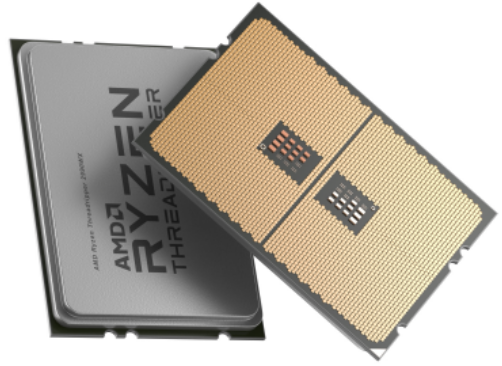
\includegraphics[width=6cm]{img/ryzen.png}
	\caption{catzo e palle}
\end{figure}

\end{multicols}
	
	\chapter{Metodo di Jacobi}

\subsection*{Introduzione}

Consideriamo il sistema lineare

\begin{equation}
	A \boldsymbol{\phi} = \boldsymbol{s}
\end{equation}

dove $A \in \mathbb{R}^{n \times n}$ è una matrice assegnata, $\boldsymbol{\phi}$ il vettore incognito e $\boldsymbol{s}$ il termine noto.

Il metodo di Jacobi si basa sulla decomposizione della matrice $A$ nella forma

\begin{equation}
	A = D - E
\end{equation}

dove: $D$ è la matrice diagonale contenente gli elementi diagonali di $A$ mentre $E$ contiene l'opposto degli elementi fuori diagonale di $A$.

Sostituendo nella relazione iniziale si ottiene:

\begin{equation}
	D \boldsymbol{\phi} = E \boldsymbol{\phi} + \boldsymbol{s}
\end{equation}

Assumendo che $D$ sia invertibile (cioè $a_{ii} \neq 0$ per ogni $i$), si può scrivere

\begin{equation}
	\boldsymbol{\phi} = D^{-1} E \boldsymbol{\phi} + D^{-1} \boldsymbol{s}
\end{equation}

Introducendo le definizioni

\begin{equation}
	H = D^{-1} E, \qquad \boldsymbol{q} = D^{-1} \boldsymbol{s}
\end{equation}

il sistema assume la forma

\begin{equation}
	\boldsymbol{\phi} = H \boldsymbol{\phi} + \boldsymbol{q}
\end{equation}

\subsection*{Struttura della matrice di iterazione}

Dalla struttura di $D$ ed $E$ si ottiene che la matrice $H$ ha forma

\begin{equation}
	H =
	\begin{pmatrix}
		0 & -\frac{a_{12}}{a_{11}} & -\frac{a_{13}}{a_{11}} & \cdots & -\frac{a_{1n}}{a_{11}} \\
		-\frac{a_{21}}{a_{22}} & 0 & -\frac{a_{23}}{a_{22}} & \cdots & -\frac{a_{2n}}{a_{22}} \\
		\vdots & \vdots & \vdots & & \vdots \\
		-\frac{a_{n1}}{a_{nn}} & -\frac{a_{n2}}{a_{nn}} & -\frac{a_{n3}}{a_{nn}} & \cdots & 0
	\end{pmatrix}
\end{equation}

Gli elementi diagonali sono nulli.

Se la matrice $A$ è diagonalmente dominante, vale

\begin{equation}
	\sum_{j=1}^{n} |h_{ij}| < 1 \quad \forall i
\end{equation}

da cui segue

\begin{equation}
	\|H\|_\infty < 1 \quad \Rightarrow \quad \rho(H) < 1
\end{equation}

Quindi la matrice $H$ è convergente.

\subsection*{Procedimento iterativo}

Si introduce il processo iterativo

\begin{equation}
	\boldsymbol{\phi}^{(m+1)} = H \boldsymbol{\phi}^{(m)} + \boldsymbol{q}
\end{equation}

con condizione iniziale

\begin{equation}
	\boldsymbol{\phi}^{(1)} = \boldsymbol{q}
\end{equation}

Esplicitando le iterazioni:

\begin{align}
	\boldsymbol{\phi}^{(2)} &= H \boldsymbol{\phi}^{(1)} + \boldsymbol{q} = H \boldsymbol{q} + \boldsymbol{q} \\
	\boldsymbol{\phi}^{(3)} &= H^2 \boldsymbol{q} + H \boldsymbol{q} + \boldsymbol{q} \\
	\vdots \\
	\boldsymbol{\phi}^{(m+1)} &= H^m \boldsymbol{q} + H^{m-1} \boldsymbol{q} + \cdots + \boldsymbol{q}
\end{align}

\subsection*{Convergenza del metodo}

Moltiplicando per $(I - H)$ si ottiene

\begin{equation}
	(I - H)\boldsymbol{\phi}^{(m+1)} = (I - H^{m+1}) \boldsymbol{q}
\end{equation}

e quindi

\begin{equation}
	\boldsymbol{\phi}^{(m+1)} = (I - H)^{-1} (I - H^{m+1}) \boldsymbol{q}
\end{equation}

Passando al limite

\begin{equation}
	\lim_{m \to \infty} \boldsymbol{\phi}^{(m+1)} = (I - H)^{-1} \boldsymbol{q}
\end{equation}

D'altra parte, la soluzione esatta soddisfa

\begin{equation}
	\boldsymbol{\phi} = H \boldsymbol{\phi} + \boldsymbol{q}
\end{equation}

da cui

\begin{equation}
	(I - H)\boldsymbol{\phi} = \boldsymbol{q}
	\quad \Rightarrow \quad
	\boldsymbol{\phi} = (I - H)^{-1} \boldsymbol{q}
\end{equation}

Quindi

\begin{equation}
	\lim_{m \to \infty} \boldsymbol{\phi}^{(m)} = \boldsymbol{\phi}
\end{equation}

\subsection*{Studio della convergenza tramite autovalori}

Sia $H$ simmetrica. Allora esiste una matrice ortogonale $U$ tale che

\begin{equation}
	U^T H U = \Lambda
\end{equation}

dove $\Lambda = \text{diag}(\lambda_1, \dots, \lambda_n)$.

Segue che

\begin{equation}
	H \boldsymbol{u}_j = \lambda_j \boldsymbol{u}_j
\end{equation}

Gli autovettori formano una base ortonormale.

\subsection{Errore}

Definiamo l'errore

\begin{equation}
	\boldsymbol{\varepsilon}^{(m)} = \boldsymbol{\phi}^{(m)} - \boldsymbol{\phi}
\end{equation}

Si ha

\begin{equation}
	\boldsymbol{\varepsilon}^{(m)} = H^m \boldsymbol{\varepsilon}^{(0)}
\end{equation}

Sviluppando sull'autobase:

\begin{equation}
	\boldsymbol{\varepsilon}^{(0)} = \sum_{h=1}^n c_h^{(0)} \boldsymbol{\phi}_h
\end{equation}

\begin{equation}
	\boldsymbol{\varepsilon}^{(m)} = \sum_{h=1}^n c_h^{(0)} \lambda_h^m \boldsymbol{\phi}_h
\end{equation}

La convergenza avviene se e solo se

\begin{equation}
	|\lambda_h| < 1 \quad \forall h
\end{equation}

cioè

\begin{equation}
	\rho(H) < 1
\end{equation}

\subsection*{Condizioni di convergenza}

Una condizione sufficiente per la convergenza è che la matrice $A$ sia strettamente diagonalmente dominante:

\begin{equation}
	|a_{ii}| > \sum_{j \neq i} |a_{ij}|
\end{equation}

Oppure irriducibilmente diagonalmente dominante:

\begin{equation}
	|a_{ii}| \ge \sum_{j \neq i} |a_{ij}|
\end{equation}

con almeno una riga per cui la disuguaglianza è stretta.

\subsection*{Definizione di irriducibilità}

Una matrice è riducibile se esiste una matrice di permutazione $P$ tale che

\begin{equation}
	P A P^T =
	\begin{pmatrix}
		\hat{A}_{11} & \hat{A}_{12} & \cdots \\
		0 & \hat{A}_{22} & \cdots \\
		\vdots & \vdots & \ddots
	\end{pmatrix}
\end{equation}

Se ciò non è possibile, la matrice è detta irriducibile.

Una matrice è irriducibile se e solo se il suo grafo orientato è fortemente connesso.

\begin{figure}[H]
	\label{connected}
	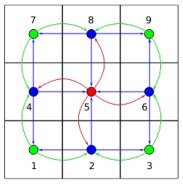
\includegraphics[width=6cm]{img/graph-connected.png}
	\caption{catzo e palle}
\end{figure}

\begin{figure}[H]
	\label{not connected}
	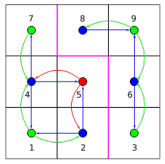
\includegraphics[width=6cm]{img/graph-not-connected.png}
	\caption{catzo e palle}
\end{figure}

\subsection*{Schema esplicito del metodo di Jacobi}

Il sistema

\begin{equation}
	\sum_{j=1}^n a_{ij} \phi_j = b_i
\end{equation}

viene risolto iterativamente come

\begin{equation}
	\phi_i^{(m+1)} =
	\frac{1}{a_{ii}}
	\left(
	b_i - \sum_{j \neq i} a_{ij} \phi_j^{(m)}
	\right)
\end{equation}

\subsection*{Implementazione per equazione di diffusione}

Nel caso bidimensionale:

\begin{equation}
	- \frac{D}{h_x^2} (\phi_{i+1,j} - 2\phi_{i,j} + \phi_{i-1,j})
	- \frac{D}{h_y^2} (\phi_{i,j+1} - 2\phi_{i,j} + \phi_{i,j-1})
	+ \Sigma_a \phi_{i,j} = Q_{i,j}
\end{equation}

Definendo

\begin{align}
	W_{i,j} = E_{i,j} &= \frac{D/h_x^2}{\Sigma_a + 2D/h_x^2 + 2D/h_y^2} \\
	S_{i,j} = N_{i,j} &= \frac{D/h_y^2}{\Sigma_a + 2D/h_x^2 + 2D/h_y^2} \\
	q_{i,j} &= \frac{Q_{i,j}}{\Sigma_a + 2D/h_x^2 + 2D/h_y^2}
\end{align}

lo schema diventa

\begin{equation}
	\phi_{i,j}^{(m+1)} =
	W_{i,j}\phi_{i-1,j}^{(m)} +
	E_{i,j}\phi_{i+1,j}^{(m)} +
	S_{i,j}\phi_{i,j-1}^{(m)} +
	N_{i,j}\phi_{i,j+1}^{(m)} +
	q_{i,j}
\end{equation}

\subsection*{Velocità di convergenza}

L'errore si comporta come

\begin{equation}
	\|\varepsilon^{(m)}\| \approx C \rho(H)^m
\end{equation}

e vale

\begin{equation}
	\lim_{m \to \infty}
	\frac{\|\varepsilon^{(m+1)}\|}{\|\varepsilon^{(m)}\|}
	= \rho(H)
\end{equation}

Il tasso asintotico di convergenza è

\begin{equation}
	R_\infty(H) = -\ln \rho(H)
\end{equation}

\subsection*{Numero di iterazioni}

Per ridurre l'errore di un fattore $\sigma$:

\begin{equation}
	\rho(H)^n < \sigma
\end{equation}

da cui

\begin{equation}
	n > \frac{\ln \sigma}{\ln \rho(H)}
	= -\frac{\ln \sigma}{R_\infty(H)}
\end{equation}

\subsection*{Osservazioni finali}

Per avere una convergenza veloce è necessario che

\begin{equation}
	\rho(H) \ll 1
\end{equation}

Si osserva che:

\begin{itemize}
	\item se $\Sigma_a \to 0$, la dominanza diagonale diminuisce e $\rho(H) \to 1$;
	\item raffinando la griglia ($h_x, h_y \to 0$), $\rho(H) \to 1$;
\end{itemize}

quindi una maggiore risoluzione spaziale comporta una convergenza più lenta.

\begin{figure}[H]
	\label{jacobi}
	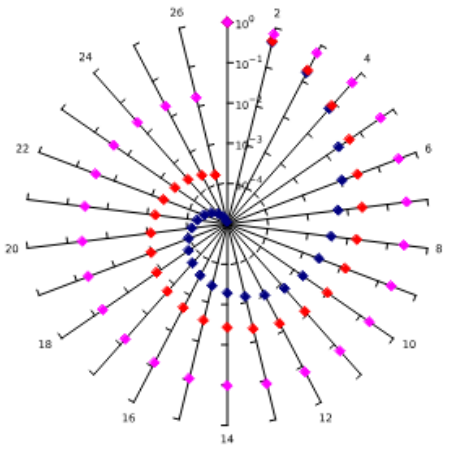
\includegraphics[width=6cm]{img/Jacobi.png}
	\caption{catzo e palle}
\end{figure}
	
	\chapter{Gauss-Siedel, SOR \& LOR}


\section{Metodo di Gauss-Seidel}

Il metodo di Jacobi calcola il flusso in ogni nodo all'iterazione $m+1$ sulla base dei flussi ottenuti all'iterazione $m$. Tuttavia, quando si aggiorna il flusso nel nodo di coordinate $(i,j)$, i nodi con indici $i$ e $j$ minori sono già stati aggiornati.

Il metodo di Gauss-Seidel cerca di sfruttare immediatamente i flussi già aggiornati nell'iterazione corrente. Per fare ciò, si immagina di decomporre ulteriormente la matrice di iterazione di Jacobi $\mathbf{H}$ come segue:

\begin{equation*}
	\mathbf{H} = \mathbf{L} + \mathbf{U} \tag{1}
\end{equation*}

dove

\[
\mathbf{L} = \left[ \begin{array}{c c c c c}
	0 & 0 & 0 & \circ & 0 \\
	- \frac{a_{21}}{a_{22}} & 0 & 0 & \circ & 0 \\
	- \frac{a_{31}}{a_{33}} & - \frac{a_{32}}{a_{33}} & 0 & \circ & 0 \\
	\vdots & \vdots & \vdots & \ddots & \vdots \\
	- \frac{a_{n1}}{a_{nn}} & - \frac{a_{n2}}{a_{nn}} & - \frac{a_{n3}}{a_{nn}} & \circ & 0
\end{array} \right],
\quad
\mathbf{U} = \left[ \begin{array}{c c c c c}
	0 & - \frac{a_{12}}{a_{11}} & - \frac{a_{13}}{a_{11}} & \circ & - \frac{a_{1n}}{a_{11}} \\
	0 & 0 & - \frac{a_{23}}{a_{22}} & \circ & - \frac{a_{2n}}{a_{22}} \\
	0 & 0 & 0 & \circ & - \frac{a_{3n}}{a_{33}} \\
	\vdots & \vdots & \vdots & \ddots & \vdots \\
	0 & 0 & 0 & \circ & 0
\end{array} \right].
\]

L'equazione di iterazione assume la nuova forma:

\begin{equation*}
	\mathbf{\phi} = \mathbf{H} \mathbf{\phi} + \mathbf{q} 
	\qquad \Rightarrow \qquad \mathbf{\phi} = \mathbf{L} \mathbf{\phi} + \mathbf{U} \mathbf{\phi} + \mathbf{q} \tag{2}
\end{equation*}

che, scritta in termini di componenti,

\begin{equation}
	\phi_i = \sum_{j=1}^{i-1} l_{i,j} \phi_j + \sum_{j=i+1}^n u_{i,j} \phi_j + q_i \tag{3}
\end{equation}

permette di impostare il seguente schema iterativo:

\begin{equation}
	\mathbf{\phi}^{(m+1)} = \mathbf{L} \mathbf{\phi}^{(m+1)} + \mathbf{U} \mathbf{\phi}^{(m)} + \mathbf{q}. \tag{4}
\end{equation}

È un dato di fatto che i flussi nella prima somma dell'Eq.(3) appartengono a nodi che sono già stati aggiornati nel corso dell'iterazione $(m+1)$.

Partendo dall'Eq.(4), si ottiene:

\[ \begin{aligned}
\mathbf{\phi}^{(m+1)} &= \mathbf{L} \mathbf{\phi}^{(m+1)} + \mathbf{U} \mathbf{\phi}^{(m)} + \mathbf{q}\ \ ,\\
(\mathbf{I} - \mathbf{L}) \mathbf{\phi}^{(m+1)} &= \mathbf{U} \mathbf{\phi}^{(m)} + \mathbf{q}\ \ ,\\
\mathbf{\phi}^{(m+1)} &= (\mathbf{I} - \mathbf{L})^{-1} \mathbf{U} \mathbf{\phi}^{(m)} + (\mathbf{I} - \mathbf{L})^{-1} \mathbf{q}\ \ . 
\end{aligned}\]

La matrice di iterazione di Gauss-Seidel è quindi: $\boxed{\mathbf{H}_{GS} = (\mathbf{I} - \mathbf{L})^{-1} \mathbf{U}}$ .

È possibile dimostrare che il raggio spettrale di \(\mathbf{H}_{GS}\) è legato a quello della matrice di Jacobi \(\mathbf{H}_J\) dalla relazione:

\[
\boxed{\,\rho(\mathbf{H}_{GS}) = \left[ \rho(\mathbf{H}_J) \right]^2\,}\ \ \ . 
\]

\subsubsection{Velocità di convergenza}

Nel caso del metodo di Gauss-Seidel, la velocità asintotica di convergenza è data da:

\[
R_{\infty}^{GS}\ =\ -\,\ln \rho(\mathbf{H}_{GS})\ =\ -\,2\, \ln \rho(\mathbf{H}_J)\ =\ 2\, R_{\infty}^{J}, 
\]

dove \(R_{\infty}^{J}\) è la velocità asintotica di convergenza del metodo di Jacobi.

Di conseguenza, il metodo di Gauss-Seidel converge più rapidamente del metodo di Jacobi, richiedendo circa la metà delle iterazioni.

\subsubsection{Implementazione pratica del metodo di Gauss-Seidel}

\begin{multicols}{2}
Il calcolo del flusso in ogni nodo coinvolge sia i valori dell'iterazione precedente che quelli dell'iterazione corrente. Ad esempio come si vede in figura di fianco, quando si aggiorna il flusso del nodo 10, per i nodi 4 e 9 si utilizzano i valori già aggiornati nell'iterazione corrente, mentre per i nodi 11 e 16 si adottano quelli dell'iterazione precedente.

\begin{figure}[H]
	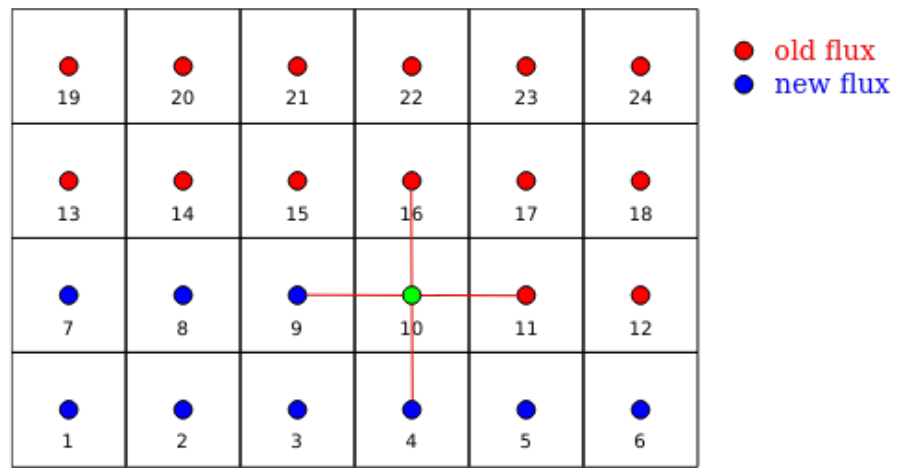
\includegraphics[width=7cm]{img/gs1.png}
	\label{gauss siedel 1}
	\caption{visualizzazione di Gauss-Siedel}
\end{figure}
\end{multicols}

Introducendo come per il metodo di Jacobi i coefficienti \(W_{i,j}\), \(E_{i,j}\), \(S_{i,j}\), \(N_{i,j}\) e il termine sorgente \(q_{i,j}\), lo schema iterativo può essere espresso come:

\[
\phi_{i,j}^{(m+1)} = W_{i,j} \phi_{i-1,j}^{(m+1)} + E_{i,j} \phi_{i+1,j}^{(m)} + S_{i,j} \phi_{i,j-1}^{(m+1)} + N_{i,j} \phi_{i,j+1}^{(m)} + q_{i,j}. \tag{9}
\]

\section{Metodo di Successive Overrelaxation (SOR)}

Il concetto di questo metodo è quello di estrapolare la previsione di Gauss-Seidel utilizzando un opportuno fattore di overrelaxation \(\omega > 1\). Partendo dalla stima di Gauss-Seidel all'iterazione \((m+1)\), Eq.(4), si sottrae \(\mathbf{\phi}^{(m)}\) da entrambi i membri:

\[
\mathbf{\phi}^{(m+1)} - \mathbf{\phi}^{(m)} = \mathbf{L} \mathbf{\phi}^{(m+1)} + (\mathbf{U} - \mathbf{I}) \mathbf{\phi}^{(m)} + \mathbf{q}\ \ . 
\]

Il flusso alla nuova iterazione \((m+1)\) viene quindi calcolato come:

\[
\mathbf{\phi}^{(m+1)} = \mathbf{\phi}^{(m)} + \omega \left[ \mathbf{\phi}^{(m+1)} - \mathbf{\phi}^{(m)} \right]_{GS},
\]

che, sostituendo l'Eq.(10), diventa:

\[
\mathbf{\phi}^{(m+1)} = \mathbf{\phi}^{(m)} + \omega \left[ \mathbf{L} \mathbf{\phi}^{(m+1)} + (\mathbf{U} - \mathbf{I}) \mathbf{\phi}^{(m)} + \mathbf{q} \right].
\]

Riorganizzando i termini, si ottiene:

\[
\mathbf{\phi}^{(m+1)} = \omega \mathbf{L} \mathbf{\phi}^{(m+1)} + \left[ (1 - \omega) \mathbf{I} + \omega \mathbf{U} \right] \mathbf{\phi}^{(m)} + \omega \mathbf{q}\ \ . 
\]

---

\subsection{Matrice di iterazione del metodo SOR}

Dall'Eq.(11) è possibile ricavare la matrice di iterazione dello schema iterativo SOR:

\[
\mathbf{\phi}^{(m+1)} = \left( \mathbf{I} - \omega \mathbf{L} \right)^{-1} \left[ (1 - \omega) \mathbf{I} + \omega \mathbf{U} \right] \mathbf{\phi}^{(m)} + \omega \left( \mathbf{I} - \omega \mathbf{L} \right)^{-1} \mathbf{q}\ \ . 
\]

La matrice di iterazione \(\mathbf{H}\) del metodo SOR è quindi:

\[
\mathbf{H} = \left( \mathbf{I} - \omega \mathbf{L} \right)^{-1} \left[ (1 - \omega) \mathbf{I} + \omega \mathbf{U} \right]\ \ . 
\]

È possibile dimostrare che esiste un valore ottimale di \(\omega\) che minimizza il raggio spettrale di \(\mathbf{H}\), dato da:

\[
\omega_{opt} = \frac{2}{1 + \sqrt{1 - \rho^2(\mathbf{H}_J)}}, \quad 1 \leq \omega_{opt} \leq 2\ \ . 
\]

Per calcolare \(\omega_{opt}\) è necessario conoscere il raggio spettrale della matrice di iterazione di Jacobi \(\mathbf{H}_J\).

\subsubsection{Stima del raggio spettrale di Jacobi}

Prima di avviare il processo iterativo SOR, è consigliabile eseguire un certo numero di iterazioni di Jacobi per ottenere una stima del suo raggio spettrale, \(\rho_{\mathbf{H}_J}\).

Consideriamo una matrice simmetrica \(\mathbf{H}_J\). Il vettore noto \(\mathbf{q}\) può essere espresso in termini degli autovettori di \(\mathbf{H}_J\) (che rappresentano una base ortogonale completa):

\[
\mathbf{q} = \sum_{h=1}^{n} q_h \mathbf{\varphi}_h\ \ . 
\]

Inoltre, ricordiamo che gli autovettori sono ortonormali, poiché \(\mathbf{U}^T \mathbf{U} = \mathbf{I}\).

---

\subsubsection{Derivazione della stima}

Si ha quindi:

\[
\begin{aligned}
	\left\| \mathbf{H}_J^m \mathbf{q} \right\|^2 &= \left( \mathbf{H}_J^m \mathbf{q}, \mathbf{H}_J^m \mathbf{q} \right) \\
	&= \left( \sum_{h=1}^{n} q_h \lambda_h^m \mathbf{\varphi}_h, \sum_{k=1}^{n} q_k \lambda_k^m \mathbf{\varphi}_k \right) \\
	&= \sum_{h=1}^{n} |q_h|^2 \lambda_h^{2m} \\
	&= \sum_{\substack{h: \\ |\lambda_h| = \rho_{\mathbf{H}_J}}}^n |q_h|^2 \rho_{\mathbf{H}_J}^{2m} + \sum_{\substack{h: \\ |\lambda_h| < \rho_{\mathbf{H}_J}}}^n |q_h|^2 \lambda_h^{2m} \\
	&= \rho_{\mathbf{H}_J}^{2m} \left[ \sum_{\substack{h: \\ |\lambda_h| = \rho_{\mathbf{H}_J}}}^n |q_h|^2 + \sum_{\substack{h: \\ |\lambda_h| < \rho_{\mathbf{H}_J}}}^n |q_h|^2 \frac{\lambda_h^{2m}}{\rho_{\mathbf{H}_J}^{2m}} \right]\ \ . 
\end{aligned}
\]

Consideriamo ora il seguente limite:

\[
\lim_{m \to \infty} \frac{\left\| \mathbf{H}_J^{m+1} \mathbf{q} \right\|^2}{\left\| \mathbf{H}_J^m \mathbf{q} \right\|^2}\ \ . 
\]

Dall'Eq.(16), per \(m \to \infty\), i rapporti nella sommatoria per \(h: |\lambda_h| < \rho_{\mathbf{H}_J}\) tenderanno tutti a zero, così che l'Eq.(17) si riduce a:

\[
\lim_{m \to \infty} \frac{\left\| \mathbf{H}_J^{m+1} \mathbf{q} \right\|^2}{\left\| \mathbf{H}_J^m \mathbf{q} \right\|^2} = \lim_{m \to \infty} \frac{\rho_{\mathbf{H}_J}^{2m+2}}{\rho_{\mathbf{H}_J}^{2m}} \frac{\sum_{h: |\lambda_h| = \rho_{\mathbf{H}_J}} |q_h|^2}{\sum_{h: |\lambda_h| = \rho_{\mathbf{H}_J}} |q_h|^2} = \rho_{\mathbf{H}_J}^2\ \ . 
\]

---

\subsection{Applicazione pratica}

In pratica, ricordando che:

\[
\mathbf{\phi}^{(m+1)} = \mathbf{H}_J \mathbf{\phi}^{(m)} + \mathbf{q} = \mathbf{H}_J^m \mathbf{q} + \mathbf{H}_J^{m-1} \mathbf{q} + \dots + \mathbf{q}\ \ , 
\]

si ha:

\[
\left\| \mathbf{\phi}^{(m+1)} - \mathbf{\phi}^{(m)} \right\| = \left\| \mathbf{H}_J^m \mathbf{q} \right\|\ \ . 
\]

Dall'Eq.(18), segue che:

\[
\lim_{m \to \infty} \frac{\left\| \mathbf{H}_J^{m+1} \mathbf{q} \right\|}{\left\| \mathbf{H}_J^m \mathbf{q} \right\|} = \lim_{m \to \infty} \frac{\left\| \mathbf{\phi}^{(m+2)} - \mathbf{\phi}^{(m+1)} \right\|}{\left\| \mathbf{\phi}^{(m+1)} - \mathbf{\phi}^{(m)} \right\|} = \rho_{\mathbf{H}_J}\ \ . 
\]

\begin{multicols}{2}
Pertanto, vengono eseguite diverse iterazioni di Jacobi fino a quando il rapporto \(\frac{\left\| \mathbf{\phi}^{(m+2)} - \mathbf{\phi}^{(m+1)} \right\|}{\left\| \mathbf{\phi}^{(m+1)} - \mathbf{\phi}^{(m)} \right\|}\) non viene considerato una stima sufficientemente accurata del raggio spettrale.

Inoltre si può mostrare che $\omega=\omega_{opt}$:
\[\rho_{\mathbf H_{SOR}}\ =\ \frac{2}{1+\sqrt{1-\rho^2_{\mathbf H_J}}}\,-\,1\]

\begin{figure}[H]
	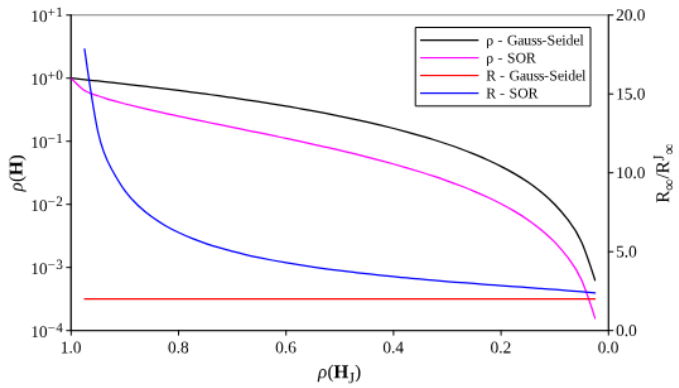
\includegraphics[width=5cm]{img/gs3.png}
	\label{SOR}
	\caption{Gauss-Siedel vs}
\end{figure}
\end{multicols}

\section{Implementazione pratica del metodo SOR}

Riprendendo l'Eq.(11),

\[
\mathbf{\phi}^{(m+1)} = \omega \mathbf{L} \mathbf{\phi}^{(m+1)} + \left[ (1 - \omega) \mathbf{I} + \omega \mathbf{U} \right] \mathbf{\phi}^{(m)} + \omega \mathbf{q},
\]

e riscrivendola in termini di componenti, si ottiene:

\[
\phi_i^{(m+1)} = \omega \sum_{j=1}^{i-1} l_{i,j} \phi_j^{(m+1)} + (1 - \omega) \phi_i^{(m)} + \omega \sum_{j=i+1}^n u_{i,j} \phi_j^{(m)} + \omega q_i\ \ . 
\]

Per un dominio 2D, utilizzando una notazione a doppio indice e introducendo i coefficienti \(W_{i,j}\), \(E_{i,j}\), \(S_{i,j}\), \(N_{i,j}\), si ha:

\[
\begin{aligned}
	\phi_{i,j}^{(m+1)} &= (1 - \omega) \phi_{i,j}^{(m)} + \omega W_{i,j} \phi_{i-1,j}^{(m+1)} + \omega S_{i,j} \phi_{i,j-1}^{(m+1)} \\
	&\quad + \omega E_{i,j} \phi_{i+1,j}^{(m)} + \omega N_{i,j} \phi_{i,j+1}^{(m)} + \omega q_{i,j}. 
\end{aligned}
\]

---

\section{Strategia iterativa Red \& Black}

Sia il metodo di Gauss-Seidel che il metodo SOR possono implementare una strategia di scansione particolare chiamata \textbf{Red \& Black}.

\paragraph{Passo 1: Aggiornamento dei nodi rossi}

In questa fase, vengono aggiornati solo i nodi \textit{rossi}:

\[
\phi_{i,j}^{(m+1)} = W_{i,j} \phi_{i-1,j}^{(m)} + E_{i,j} \phi_{i+1,j}^{(m)} + S_{i,j} \phi_{i,j-1}^{(m)} + N_{i,j} \phi_{i,j+1}^{(m)} + q_{i,j}. 
\]

\paragraph{Passo 2: Aggiornamento dei nodi neri}

In questa fase, vengono aggiornati solo i nodi \textit{neri}:

\[
\phi_{i,j}^{(m+1)} = W_{i,j} \phi_{i-1,j}^{(m+1)} + E_{i,j} \phi_{i+1,j}^{(m+1)} + S_{i,j} \phi_{i,j-1}^{(m+1)} + N_{i,j} \phi_{i,j+1}^{(m+1)} + q_{i,j}. 
\]

Questa strategia consente un trattamento più coerente di ogni nodo, evitando la generazione di componenti asimmetriche spurie nell'errore. Nella valutazione del flusso in ogni nodo, i flussi dei nodi vicini appartengono tutti alla stessa iterazione.

\begin{multicols}{2}
\begin{figure}[H]
	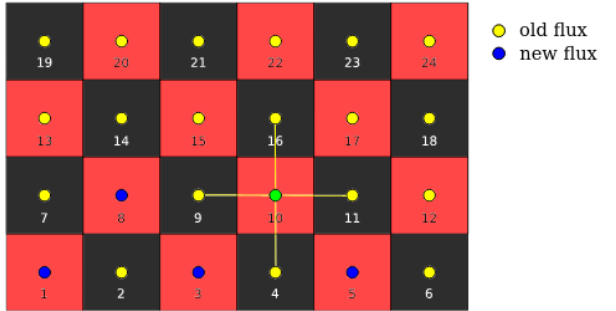
\includegraphics[width=7cm]{img/gs4.png}
	\label{red}
	\caption{step 1 del metodo Red \& Black}
\end{figure}

\begin{figure}[H]
	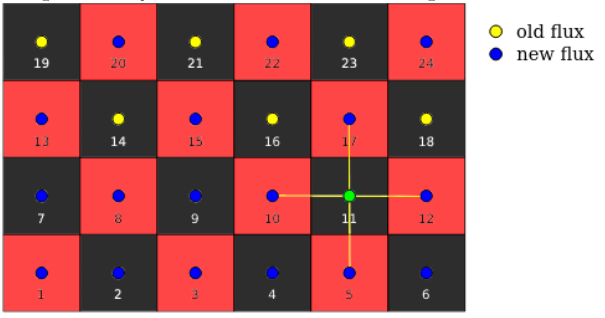
\includegraphics[width=7cm]{img/gs5.png}
	\label{and black}
	\caption{step 2 del metodo Red \& Black}
\end{figure}
\end{multicols}

\section{Metodo Line Overrelaxation (LOR)}

Facciamo riferimento al dominio 2D mostrato in figura. La matrice dei coefficienti \(\mathbf{A}\) del sistema di equazioni nodali può essere letta come una matrice a blocchi (3x3), i cui blocchi diagonali (in blu) sono matrici tridiagonali.

\[
\left[ \begin{array}{l l l l l l l l l}
	a_{11} & a_{12} & 0 & a_{14} & 0 & 0 & 0 & 0 & 0 \\
	a_{21} & a_{22} & a_{23} & 0 & a_{25} & 0 & 0 & 0 & 0 \\
	0 & a_{32} & a_{33} & 0 & 0 & a_{36} & 0 & 0 & 0 \\
	a_{41} & 0 & 0 & a_{44} & a_{45} & 0 & a_{47} & 0 & 0 \\
	0 & a_{52} & 0 & a_{54} & a_{55} & a_{56} & 0 & a_{58} & 0 \\
	0 & 0 & a_{63} & 0 & a_{65} & a_{66} & 0 & 0 & a_{69} \\
	0 & 0 & 0 & a_{74} & 0 & 0 & a_{77} & a_{78} & 0 \\
	0 & 0 & 0 & 0 & a_{85} & 0 & a_{87} & a_{88} & a_{89} \\
	0 & 0 & 0 & 0 & 0 & a_{96} & 0 & a_{98} & a_{99}
\end{array} \right]
\left[ \begin{array}{l}
	\phi_1 \\ \phi_2 \\ \phi_3 \\ \phi_4 \\ \phi_5 \\ \phi_6 \\ \phi_7 \\ \phi_8 \\ \phi_9
\end{array} \right]
=
\left[ \begin{array}{l}
	s_1 \\ s_2 \\ s_3 \\ s_4 \\ s_5 \\ s_6 \\ s_7 \\ s_8 \\ s_9
\end{array} \right]\ \ . 
\]

La matrice può essere riscritta in forma a blocchi:

\[
\left[ \begin{array}{l l l}
	\hat{\mathbf{A}}_{11} & \hat{\mathbf{A}}_{12} & 0 \\
	\hat{\mathbf{A}}_{21} & \hat{\mathbf{A}}_{22} & \hat{\mathbf{A}}_{23} \\
	0 & \hat{\mathbf{A}}_{32} & \hat{\mathbf{A}}_{33}
\end{array} \right]
\left[ \begin{array}{l}
	\hat{\mathbf{\phi}}_1 \\ \hat{\mathbf{\phi}}_2 \\ \hat{\mathbf{\phi}}_3
\end{array} \right]
=
\left[ \begin{array}{l}
	\hat{\mathbf{s}}_1 \\ \hat{\mathbf{s}}_2 \\ \hat{\mathbf{s}}_3
\end{array} \right]\ \ . 
\]

---

\subsubsection{Equazione generica del sistema}

L'equazione generica del sistema (28), scritta in forma a blocchi, è:

\[
\hat{\mathbf{A}}_{i,i-1} \hat{\mathbf{\phi}}_{i-1} + \hat{\mathbf{A}}_{i,i} \hat{\mathbf{\phi}}_i + \hat{\mathbf{A}}_{i,i+1} \hat{\mathbf{\phi}}_{i+1} = \hat{\mathbf{s}}_i\ \ . 
\]

Il primo termine riguarda i flussi della riga \(i-1\), mentre il terzo termine riguarda i flussi della riga \(i+1\). Quando si trattano i nodi della \(i\)-esima riga, quelli sulla riga \(i-1\) sono già stati calcolati. Si può quindi adottare una strategia simile a Gauss-Seidel:

\[
\hat{\mathbf{A}}_{i,i} \hat{\mathbf{\phi}}_i^{(m+1)} = \hat{\mathbf{s}}_i - \hat{\mathbf{A}}_{i,i-1} \hat{\mathbf{\phi}}_{i-1}^{(m+1)} - \hat{\mathbf{A}}_{i,i+1} \hat{\mathbf{\phi}}_{i+1}^{(m)}\ \ . 
\]

L'equazione sopra è un **sistema tridiagonale** che può essere risolto efficientemente con l'algoritmo di Thomas.

---

\subsection*{Introduzione dell'overrelaxation}

Come fatto per il metodo SOR, anche qui possiamo introdurre un'overrelaxation, scrivendo:

\[
\hat{\mathbf{A}}_{i,i} \hat{\mathbf{\phi}}_i^{(m+1)} = \hat{\mathbf{A}}_{i,i} \hat{\mathbf{\phi}}_i^{(m)} + \omega \left[ \hat{\mathbf{A}}_{i,i} \hat{\mathbf{\phi}}_i^{(m+1)} - \hat{\mathbf{A}}_{i,i} \hat{\mathbf{\phi}}_i^{(m)} \right]_{GS}\ \ . 
\]

Grazie all'Eq.(30), possiamo sostituire il primo termine tra parentesi per ottenere:

\[
\hat{\mathbf{A}}_{i,i} \hat{\mathbf{\phi}}_i^{(m+1)} = \omega \hat{\mathbf{s}}_i - \omega \hat{\mathbf{A}}_{i,i-1} \hat{\mathbf{\phi}}_{i-1}^{(m+1)} - \omega \hat{\mathbf{A}}_{i,i+1} \hat{\mathbf{\phi}}_{i+1}^{(m)} + (1 - \omega) \hat{\mathbf{A}}_{i,i} \hat{\mathbf{\phi}}_i^{(m)}\ \ . 
\]

Anche in questo caso, il lato destro è un termine noto, mentre la matrice \(\hat{\mathbf{A}}_{i,i}\) è tridiagonale.

---

\subsection*{Implementazione pratica del metodo LOR}

Con riferimento alla figura precedente e adottando una notazione a doppio indice, possiamo scrivere:

\[
\begin{array}{l}
	W_{i,j} \phi_{i-1,j}^{(m+1)} + O_{i,j} \phi_{i,j}^{(m+1)} + E_{i,j} \phi_{i+1,j}^{(m+1)} = -\omega S_{i,j} \phi_{i,j-1}^{(m+1)} - \omega N_{i,j} \phi_{i,j+1}^{(m)} \\
	\quad + \omega q_{i,j} + (1 - \omega) \left[ W_{i,j} \phi_{i-1,j}^{(m)} + O_{i,j} \phi_{i,j}^{(m)} + E_{i,j} \phi_{i+1,j}^{(m)} \right]\ \ . 
\end{array}
\]

È un'equazione a tre punti. Procedendo per colonne, l'Eq.(33) diventa:

\[
\begin{array}{l}
	S_{i,j} \phi_{i,j-1}^{(m+1)} + O_{i,j} \phi_{i,j}^{(m+1)} + N_{i,j} \phi_{i,j+1}^{(m+1)} = -\omega W_{i,j} \phi_{i-1,j}^{(m+1)} - \omega E_{i,j} \phi_{i+1,j}^{(m)} \\
	\quad + \omega q_{i,j} + (1 - \omega) \left[ S_{i,j} \phi_{i,j-1}^{(m)} + O_{i,j} \phi_{i,j}^{(m)} + N_{i,j} \phi_{i,j+1}^{(m)} \right]\ \ .
\end{array}
\]


\begin{figure}[H]
	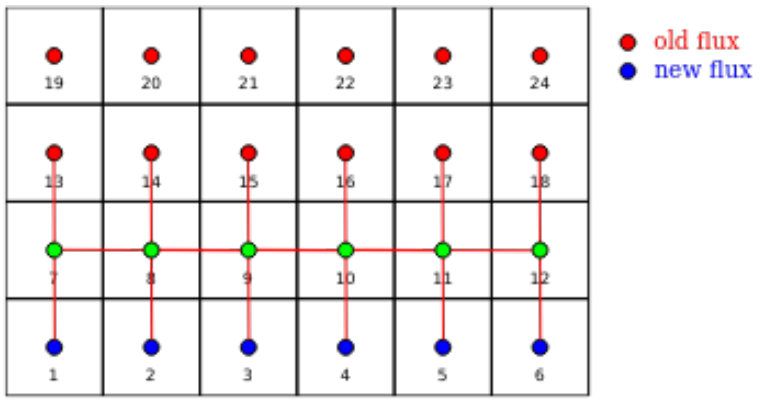
\includegraphics[width=5cm]{img/gs6.png}
	\label{  }
	\caption{  }
\end{figure}
	
	\chapter{Alternate direction implicit}


\begin{figure}[H]
	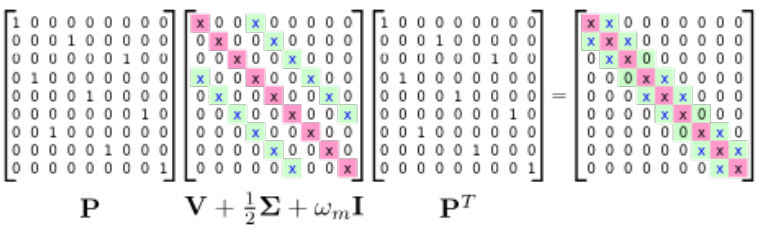
\includegraphics[width=5cm]{img/exampleADI.png}
	\label{  }
	\caption{  }
\end{figure}
	
	\chapter{Metodi del gradiente}

I metodi del gradiente costituiscono una classe di metodi iterativi utilizzati per risolvere sistemi lineari della forma

\begin{equation*}
	A x = b,
\end{equation*}

dove $A \in \mathbb{R}^{n \times n}$ è una matrice simmetrica definita positiva (SPD).

Ricordiamo che una matrice simmetrica è definita positiva se vale la proprietà

\begin{equation*}
	v^T A v\ =\ (Av, v)\, >\, 0 \qquad \forall\ v \neq \{0\}\ \ .
\end{equation*}

Nota che la scrittura $v^T A v\ =\ (Av, v)$ è vera perché \textbf{A} è simmetrica, altrimenti se non lo fosse $(Av, v)$ si svilupperebbe come $(Av)^T v=v^T A^T v$, che non è chiaramente la stessa cosa.

\section{Formulazione variazionale del problema}

Sia $x = \phi$ la soluzione del sistema lineare $Ax = b$. 

Si può dimostrare che tale soluzione coincide con il minimo del funzionale quadratico

\begin{equation*}
	F(x) = \frac{1}{2}(Ax, x) - (b, x).
\end{equation*}

Per cui vale la relazione:

\begin{equation*}
	F(\phi)\ =\ \min_{x} F(x)\ \ .
\end{equation*}

\subsubsection{Dimostrazione}

Poiché $b = A\phi$, il funzionale può essere riscritto come
\begin{equation*}
	F(x)\ =\ \frac{1}{2}(Ax, x) \,-\, (A\phi, x)\ \ .
\end{equation*}

Valutando il funzionale nella soluzione esatta si ottiene

\begin{equation*}
	F(\phi)\ =\ \frac{1}{2}(A\phi, \phi)\, -\, (A\phi, \phi)\ =\ -\,\frac{1}{2}\,(A\phi, \phi)\ \ .
\end{equation*}

O, equivalentemente:

\begin{equation*}
	F(\phi)\, +\, \frac{1}{2}\,(A\phi, \phi)\ =\ 0\ \ .
\end{equation*}

Aggiungendo e sottraendo opportunamente termini, si può riscrivere $F(x)$ come

\begin{equation*}
	\begin{aligned}
		F(x)\ &=\ \frac{1}{2}(A\phi,\, \phi)\,-\,\color{blue}{(A\phi,\,  x)}\color{black}{\,+\,\underset{=0}{\underbrace{F(\phi)\,+\, \frac{1}{2}(A\phi,\,  \phi)}}\ =}\\
		&=\ F(\phi)\,+\, \frac{1}{2}(Ax,\,  x)\, \color{blue}{-\,\frac{1}{2}(A\phi, \, x)\, -\,\frac{1}{2}(A\phi,\,  x)}\color{black}{\,+\, \frac{1}{2}(A\phi,\,  \phi)\ =}\\
		&=\ F(\phi)\, +\, \frac{1}{2}\,(A(x-\phi),\, x)\, -\, \frac{1}{2}\,(A\phi, \,(x-\phi))\ =\\ 
		&=\ F(\phi)\, +\,\frac{1}{2}\,(A(x-\phi),\, x)\, -\, \frac{1}{2}\,(A(x-\phi),\, \phi)\ =\\
		&=\ F(\phi)\, +\, \frac{1}{2}\,(A(x-\phi), x-\phi) 
 .	\end{aligned}
\end{equation*}

Poiché $A$ è definita positiva, il termine $(A(x-\phi),\,  x-\phi)$ è sempre positivo per $x \neq \phi$. Ne segue che il minimo del funzionale è raggiunto esattamente per $x = \phi$.

\emph{Questo risultato mostra che la risoluzione del sistema lineare $Ax = b$ è equivalente alla minimizzazione del funzionale $F(x)$}.

\section{Interpretazione tramite errore}

Data una soluzione approssimata $x$, si possono definire diverse misure dell'errore:

\begin{equation}
	\label{errori gradiente}
	\begin{aligned}
		E_1(x)\ &=\ (\phi - x)^T\, (\phi - x)\ =\ \varepsilon^T\, \varepsilon\ , \\
		E_2(x)\ &=\ (b - Ax)^T\, (b - Ax)\ =\ r^T\, r\ , \\
		E_3(x)\ &=\ (\phi - x)^T\, (b - Ax)\ =\ \varepsilon^T\, A\, \varepsilon\ .
	\end{aligned}
\end{equation}

Indicando con $\varepsilon = \phi - x$ e osservando che $b - Ax = A\phi - Ax = A(\phi - x) = A\varepsilon$.

\emph{Tutte queste quantità sono nulle se e solo se $x = \phi$}.

%
%
\subsection{Relazione tra errore e funzionale}

Espandendo $E_3(x)$ si ottiene
\begin{align*}
	E_3(x) &= \phi^T b - \phi^T A x - x^T b + x^T A x \\
	&= \phi^T b + x^T A x - 2 x^T b\ \ .
\end{align*}

Utilizzando la definizione del funzionale $F(x)$, si ricava
\begin{equation*}
	E_3(x)\ =\ \phi^T b + 2F(x)\ .
\end{equation*}

Affinché l'errore si annulli nella soluzione esatta, deve valere
\begin{equation*}
	F(\phi)\ =\ -\frac{1}{2}\phi^T b = -\frac{1}{2}(A\phi, \phi)\ ,
\end{equation*}

che coincide con il valore minimo del funzionale.

\bigskip

In conclusione, la minimizzazione del funzionale $F(x)$ è completamente equivalente alla risoluzione del sistema lineare $Ax = b$, e fornisce la base teorica per lo sviluppo dei metodi iterativi basati sul gradiente.


\section{Metodi di discesa}

I metodi di discesa sono metodi iterativi che mirano a determinare il minimo del funzionale $F(x)$ costruendo una successione di approssimazioni $x^{(0)}, x^{(1)}, x^{(2)}, \dots$ a partire da una stima iniziale $x^{(0)}$.

L'idea fondamentale è che ogni nuova iterazione migliori la precedente, ovvero che il valore del funzionale decresca:
\begin{equation*}
	F\big(x^{(k+1)}\big) \leq F\big(x^{(k)}\big),
\end{equation*}
idealmente con disuguaglianza stretta.

Quando si raggiunge una configurazione tale che $Ax^{(k)} \approx b$, il processo può essere arrestato e $x^{(k)}$ viene considerata una buona approssimazione della soluzione.

\subsubsection{Struttura generale del metodo}

\begin{multicols}{2}
Il passaggio da $x^{(k)}$ a $x^{(k+1)}$ avviene tramite un processo in due fasi fondamentali:

\begin{enumerate}
	\item \textbf{Scelta della direzione di ricerca} $p^{(k)}$;
	\item \textbf{Scelta del passo} $\alpha_k$, che determina quanto muoversi lungo tale direzione.
\end{enumerate}

La nuova iterata è quindi definita come
\begin{equation*}
	x^{(k+1)}\ =\ x^{(k)}\, +\, \alpha_k \, p^{(k)}\  .
\end{equation*}

\begin{figure}[H]
	\centering
	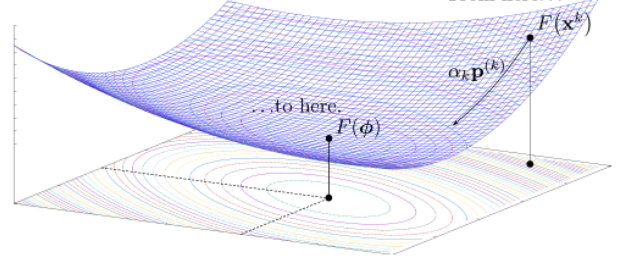
\includegraphics[width=8cm]{img/gradient1.png}
	\label{discesa}
	\caption{Visualizzazione delle grandezze definite.}
\end{figure}
\end{multicols}

Dal punto di vista matematico: $p^{(k)} \in \mathbb{R}^n$ è il vettore direzione;
$\alpha_k \in \mathbb{R}$ è un parametro scalare (step size).


\subsubsection{Scelta della direzione}

La scelta della direzione $p^{(k)}$ è cruciale per l'efficienza del metodo. Una scelta naturale per la direzione di discesa consiste nell’utilizzare il gradiente del funzionale. Infatti, la direzione in cui una funzione scalare varia più rapidamente è proprio quella del suo gradiente.

Si sceglie quindi come direzione di ricerca il negativo del gradiente:
\[\begin{aligned}
	p^{(k)}\ &=\ - \nabla\, F\big(x^{(k)}\big)\ =\ -\nabla\left[\frac{1}{2}(Ax^{(k)},\, x)\, -\, (b,\,x^{(k)})\right]\ =\\
	&=\ -\,\nabla\,\left[\frac{1}{2}\, x^{{(k)}^T}\,A\,x^{(k)}\, -\, x^{{(k)}^T}\, b\right]\ =\\
	&=\ -\, \left[\frac{1}{2} A x^{(k)} + \frac{1}{2} x^{{(k)}^T}\, A - b\right]\ \ .	
\end{aligned}\]

Poiché $A$ è simmetrica ($A = A^T$) , segue $\nabla F(x^{(k)}) = A x^{(k)} - b\,$ e, pertanto, la direzione di discesa diventa:
\begin{equation}
	\boxed{p^{(k)}\ =\ b\, -\, A x^{(k)}\ =\ r^{(k)}}\ \ ,
\end{equation}

dove $r^{(k)}$ è il \underline{residuo}, direzione lungo la quale il funzionale decresce maggiormente a partire da $x^{(k)}$.

%
%
%
\subsubsection{Scelta del passo}

Il parametro $\alpha_k$ viene scelto imponendo che il funzionale sia minimo lungo la direzione $r^{(k)}$, cioè:
\begin{equation}
	F\big(x^{(k+1)}\big) = \min_{\alpha_k} F\big(x^{(k)} + \alpha_k r^{(k)}\big).
\end{equation}

Per determinare tale valore, si impone la condizione di stazionarietà $\frac{d}{d\alpha_k} F\big(x^{(k+1)}\big) = 0$ e sostituendo $x^{(k+1)} = x^{(k)} + \alpha_k r^{(k)}$ nel funzionale si ottiene:
\begin{equation*}
	F\big(x^{(k+1)}\big)\ =\ \frac{1}{2}\, \left( A(x^{(k)} + \alpha_k r^{(k)}), \, x^{(k)}\, +\, \alpha_k r^{(k)} \right) 
	\, -\, \left( b, x^{(k)} + \alpha_k r^{(k)} \right)\ \ ,
\end{equation*}

ovvero, in forma matriciale:
\begin{equation*}
	F\big(x^{(k+1)}\big)\ =\ \frac{1}{2} (x^{(k)} + \alpha_k r^{(k)})^T A (x^{(k)}\, +\, \alpha_k r^{(k)}) 
	\, -\, (x^{(k)}\, +\, \alpha_k r^{(k)})^T\, b.
\end{equation*}

Sviluppando i termini si ottiene:
\begin{equation*}
	F\big(x^{(k+1)}\big)
	= \frac{1}{2} x^{(k)T} A x^{(k)}
	+ \alpha_k r^{(k)T} A x^{(k)}
	+ \frac{1}{2} \alpha_k^2 r^{(k)T} A r^{(k)}
	\quad - x^{(k)T} b - \alpha_k r^{(k)T} b.
\end{equation*}

Raccogliendo i termini:
\begin{equation*}
	F\big(x^{(k+1)}\big)
	= F\big(x^{(k)}\big)
	+ \alpha_k r^{(k)T} (A x^{(k)} - b)
	+ \frac{1}{2} \alpha_k^2 r^{(k)T} A r^{(k)}.
\end{equation*}

Poiché $r^{(k)} = b - A x^{(k)}$, segue:
\begin{equation*}
	F\big(x^{(k+1)}\big)
	= F\big(x^{(k)}\big)
	- \alpha_k r^{(k)T} r^{(k)}
	+ \frac{1}{2} \alpha_k^2 r^{(k)T} A r^{(k)}.
\end{equation*}

Imponendo la condizione di minimo:
\begin{equation*}
	\frac{d}{d\alpha_k} F\big(x^{(k+1)}\big)
	= - r^{(k)T} r^{(k)} + \alpha_k r^{(k)T} A r^{(k)} = 0,
\end{equation*}

da cui si ricava

\[\boxed{\,\alpha_k\ =\ \frac{r^{(k)T}\, r^{(k)}}{r^{(k)T}\, A\, r^{(k)}}\ =\ \frac{(r^{(k)},\, r^{(k)})}{(A r^{(k)},\, r^{(k)})}\, }\ \ .\]

La condizione di minimo del funzionale lungo la direzione di ricerca può essere riscritta in forma più compatta utilizzando la regola della derivazione composta. Infatti, si ha:

\begin{equation*}
	\frac{d}{d\alpha_k} F\big(x^{(k+1)}\big)
	\ =\
	\frac{dx^{(k+1)}}{d\alpha_k}
	\,\cdot\,
	\frac{dF\big(x^{(k+1)}\big)}{dx^{(k+1)}}
	\ =\ 0\ \ .
\end{equation*}

Dalla definizione dell'iterazione $x^{(k+1)} = x^{(k)} + \alpha_k r^{(k)}$, segue immediatamente che
\begin{equation*}
	\frac{dx^{(k+1)}}{d\alpha_k} = r^{(k)}.
\end{equation*}

D'altra parte, la derivata del funzionale rispetto alla variabile $x$ è il suo gradiente, quindi:
\begin{equation*}
	\frac{dF\big(x^{(k+1)}\big)}{dx^{(k+1)}} = \nabla F\big(x^{(k+1)}\big).
\end{equation*}

Ricordando che $\nabla F(x) = Ax - b = -r$, si ottiene:
\begin{equation*}
	\nabla F\big(x^{(k+1)}\big) = -r^{(k+1)}.
\end{equation*}

Sostituendo nella condizione di cui sopra, $r^{(k)} \cdot \big(-r^{(k+1)}\big) = 0$, segue la proprietà fondamentale
\begin{equation*}
	r^{(k)} r^{(k+1)} = 0 \qquad \rightarrow \quad r^{(k)}\perp r^{(k+1)} \ \ .
\end{equation*}

\subsubsection{Interpretazione}

La relazione precedente mostra che i residui di due iterazioni successive sono ortogonali tra loro.

Questa proprietà ha un significato geometrico molto importante: il passo $\alpha_k$ è scelto in modo tale che il nuovo punto $x^{(k+1)}$ sia il minimo del funzionale lungo la direzione $r^{(k)}$.

Di conseguenza:
\begin{itemize}
	\item il gradiente nel punto $x^{(k+1)}$ è ortogonale alla direzione seguita;
	\item poiché il gradiente è opposto al residuo, si ha che $r^{(k+1)}$ è ortogonale a $r^{(k)}$.
\end{itemize}

In altre parole, ogni iterazione elimina completamente la componente dell'errore lungo la direzione appena utilizzata.

Tuttavia, in generale non vale
\[
r^{(k)} r^{(j)} = 0 \quad \text{per } j \neq k \pm 1,
\]
cioè i residui non sono tutti mutuamente ortogonali, ma solo quelli consecutivi.

%
%
%
\subsection{Algoritmo del Steepest Descent Method}
Ecco lo pseudocodice che implementa il metodo, con ogni passaggio commentato:

\begin{lstlisting}[caption={Algoritmo del Steepest Descent Method}]
% Inizializzazione
x = x0;                % Stima iniziale
r = b - A * x;         % Residuo iniziale
	
% Iterazione fino a convergenza
while ||r|| > tolleranza
	
	% Calcolo del parametro alpha_k
	alpha = (r^T * r) / (r^T * A * r);
		
	% Aggiornamento della soluzione x_k -> x_{k+1}
	x = x + alpha * r;
		
	% Aggiornamento del residuo in funzione di x_{k+1}
	r = b - A * x;
	% potrebbe essere calcolato anche come 
	% b - A*x_k - alpha_k*A*r_k = r_k - alpha_k*A*r_k
end
\end{lstlisting}

\begin{itemize}
	\item \texttt{x0}: Stima iniziale della soluzione.
	\item \texttt{r}: Residuo iniziale, calcolato come \(\mathbf{b} - \mathbf{A} \mathbf{x}\).
	\item \texttt{alpha}: Parametro di passo calcolato come \(\frac{\mathbf{r}^T \mathbf{r}}{\mathbf{r}^T \mathbf{A} \mathbf{r}}\).
	\item \texttt{while ||r|| > tolleranza}: Iterazione finché il residuo non scende sotto una soglia prefissata.
	\item \texttt{x = x + alpha * r}: Aggiornamento della soluzione lungo la direzione del residuo.
	\item \texttt{r = b - A * x}: Aggiornamento del residuo dopo ogni iterazione.
\end{itemize}


%
%
%
\subsection{Interpretazione geometrica}

Data l'eq.(\eqref{errori gradiente}), dove \(\mathbf{\epsilon} = \mathbf{\phi} - \mathbf{x}\), se espandiamo \(\mathbf{\epsilon}\) in termini degli autovettori di \(\mathbf{A}\), $\mathbf{\epsilon} = \mathbf{U} \mathbf{z}$, dove \(\mathbf{U}\) è la matrice ortogonale degli autovettori e \(\mathbf{z}\) è il vettore dei coefficienti, otteniamo:

\begin{equation*}
	E_3(\mathbf{z})\ =\  (\mathbf{U} \mathbf{z})^T\, \mathbf{A}\, \mathbf{U} \mathbf{z}\ =\ \mathbf{z}^T \mathbf{U}^T\, \mathbf{A}\, \mathbf{U} \mathbf{z}\ =\ \mathbf{z}^T\, \mathbf{\Lambda}\, \mathbf{z},
\end{equation*}

con \(\mathbf{\Lambda}\) matrice diagonale degli autovalori \(\lambda_i\) di \(\mathbf{A}\).

\subsubsection{Iperellissoidi e autovalori}

L’equazione \eqref{eq:errore3} può essere riscritta come: $E_3(\mathbf{z}) = \lambda_1 z_1^2 + \lambda_2 z_2^2 + \dots + \lambda_n z_n^2$ .

I luoghi a errore costante sono rappresentati da iperellissoidi i cui semiassi sono legati agli autovalori di \(\mathbf{A}\):

\begin{equation*}
	r_i = \sqrt{\frac{E_3(\mathbf{z})}{\lambda_i}}.
\end{equation*}

La soluzione esatta \(\mathbf{\phi}\) corrisponde al centro degli iperellissoidi (dove \(E_3(\mathbf{z}) = 0\)).

\subsubsection{Visualizzazione geometrica}
Esempio tridimensionale (\(n=3\)) di iperellissoide.

Il metodo di discesa sposta \(\mathbf{x}^{(k)}\) sulla superficie $F(x)$ lungo la direzione di massima pendenza $r^{(k)}$ perpendicolare a $F(x^{(k)})$ fino al punto $x^{(k+1)}$ dove il funzionale assume il suo minimo valore lungo la direzione di spostamento.

Siccome vale l'ortogonalità dei residui successivi $r^{(k)}\perp r^{(k+1)}$, implica che, al passo \(k+1\), la direzione di discesa \(\mathbf{r}^{(k+1)}\) è perpendicolare all’iperellissoide corrispondente a $F(\mathbf{x}^{(k+1)})$ oltre che a $r^{(k)}$.

\begin{multicols}{2}
	
	\begin{figure}[H]
		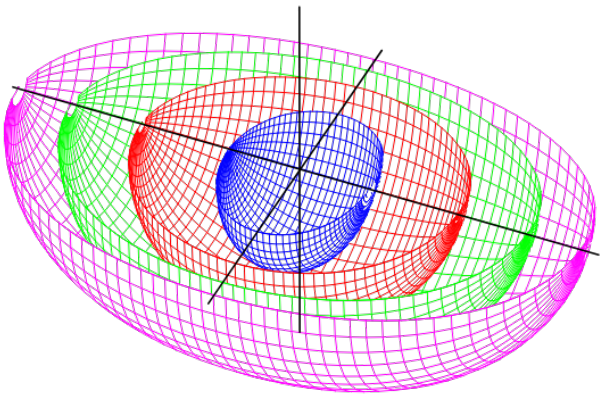
\includegraphics[width=6cm]{img/gradient2.png}
		\label{Ellissoidi}
		\caption{Visualizzazione degli ellissoidi per n=3}
	\end{figure}
	
	\begin{figure}[H]
		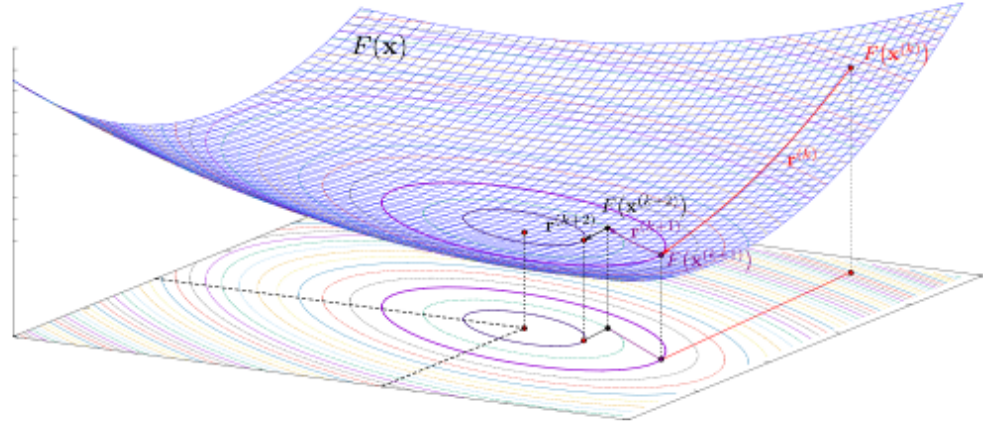
\includegraphics[width=7.5cm]{img/gradient3.png}
		\label{Discesa}
		\caption{Visualizzazione della discesa}
	\end{figure}
	
\end{multicols}
.

\begin{figure}[H]
	\centering
	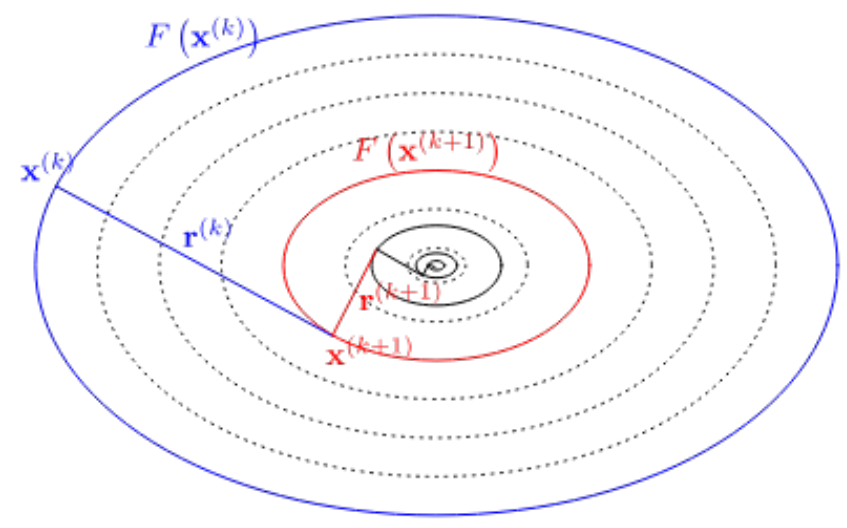
\includegraphics[width=9cm]{img/gradient4.png}
	\label{Gradient fatto bene}
	\caption{Metodo dello \emph{steepest descent} visualizzato nella sua totalità}
\end{figure}


\subsubsection{Condition number e convergenza}
Se la matrice \(\mathbf{A}\) ha numero di condizione \(\kappa(\mathbf{A}) = 1\) (cioè tutti gli autovalori sono uguali), gli iperellissoidi degenerano in ipersfere e il metodo converge in una sola iterazione, indipendentemente dal guess iniziale.

\begin{equation*}
	\kappa(\mathbf{A}) = \frac{|\lambda_{\text{max}}(\mathbf{A})|}{|\lambda_{\text{min}}(\mathbf{A})|}
\end{equation*}

\begin{multicols}{2}
\begin{figure}[H]
	\centering
	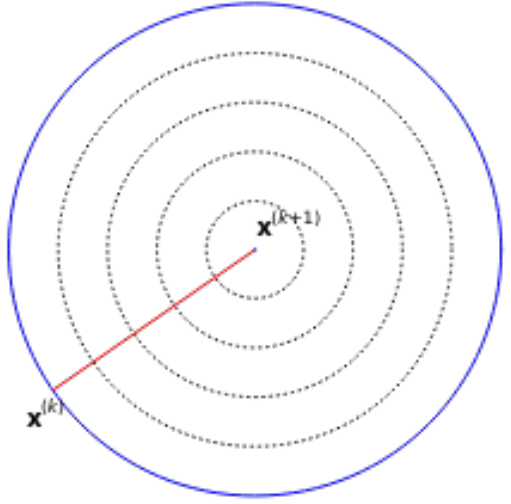
\includegraphics[width=5cm]{img/gradient5.png}
	\label{concentrici}
	\caption{Caso in cui gli iperellissoidi degenerano in ipersfere}
\end{figure}

\vspace{1cm}
\begin{figure}[H]
	\centering
	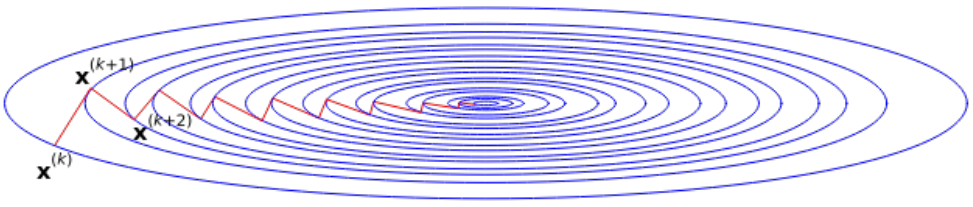
\includegraphics[width=7cm]{img/gradient6.png}
	\label{discesa lenta}
	\caption{Caso di matrice malcondizionata, che converge lentamente}
\end{figure}
\end{multicols}


Se gli autovalori sono raggruppati in un intervallo ristretto, la convergenza è veloce. Al contrario, se gli autovalori sono molto spaziati (matrice mal condizionata), la convergenza è lenta.

Se $\lambda_1 \gg \lambda_2$, l'iperellissoide è molto allungato lungo la direzione corrispondente a $\lambda_1$.
Il metodo di discesa "oscilla" tra le direzioni principali, rallentando la convergenza, come si vede in fig.(\ref{discesa lenta}).


%
%
%
\section{Conjugate Gradient Method}

Il metodo di Steepest Descent può essere lento, soprattutto per matrici mal condizionate, nel senso che può tornare spesso a muoversi in direzioni già usate in step precedenti. 

Il \underline{\emph{Conjugate Gradient Method}} è un algoritmo più efficiente che sfrutta direzioni di ricerca linearmente indipendenti.
L'algoritmo è simile a quello di Steepest Descent, ma la direzione di ricerca $\mathbf{p}^{(k)}$ è aggiornata come:

\begin{equation*}
	\mathbf{p}^{(k)} = \mathbf{r}^{(k)} + \beta_k \mathbf{p}^{(k-1)},
\end{equation*}

dove $\beta_k$ è scelto per garantire l'$\mathbf{A}$-ortogonalità:
$(\mathbf A \mathbf p^{(k-1)}, \mathbf p^{(k)}) = \mathbf{p}^{(k)^T} \mathbf{A} \mathbf{p}^{(k-1)} = 0$ .


\subsubsection{Calcolo di $\beta_k$ e del passo $\alpha_k$}

Imponendo la condizione di coniugazione, si ottiene:

\[
(\mathbf A \mathbf p^{(k-1)}, \mathbf{r}^{(k)} + \beta_k \mathbf{p}^{(k-1)})\ =\ 0
\]

\begin{equation*}
	\beta_k = -\frac{\mathbf{r}^{(k)^T} \mathbf{A} \mathbf{p}^{(k-1)}}{\mathbf{p}^{(k-1)^T} \mathbf{A} \mathbf{p}^{(k-1)}}.
\end{equation*}

L'insieme di direzioni di ricerca $\mathbf p^{(k)}$ così ottenuto formano un insieme di vettori linearmente indipendenti.

Il parametro \(\alpha_k\) è scelto per minimizzare \(F(\mathbf{x}^{(k+1)})\) lungo \(\mathbf{p}^{(k)}\):

\[\begin{aligned}
F(\mathbf{x}^{(k+1)})\ &=\ 
\frac{1}{2}\, (\mathbf A (\mathbf x^{(k)}+\alpha_k \mathbf p^{(k)}),\, (\mathbf x^{(k)}+\alpha_k \mathbf p^{(k)}))\, -\, (\mathbf b, \, (\mathbf x^{(k)}+\alpha_k \mathbf p^{(k)}))\ =\\
&=\ F(\mathbf x^{(k)})\, -\, \alpha_k \mathbf p^{(k)^T} \mathbf r^{(k)}\, +\, \frac{1}{2}\alpha_k^2 \mathbf{p}^{(k)^T} \mathbf A \mathbf p^{(k)}\ \ ,
\end{aligned}\]

\[
\frac{d\, F(\mathbf x^{(k+1)})}{d\, \alpha_k}\ =\ 0
\qquad \rightarrow \qquad
-\, \mathbf p^{(k)^T} \mathbf{r}^{(k)}\, +\, \alpha_k \mathbf{p}^{(k)^T} \mathbf A \mathbf p^{(k)}\ =\ 0\ \ ,
\]

\begin{equation*}
	\alpha_k = \frac{\mathbf{p}^{(k)^T} \mathbf{r}^{(k)}}{\mathbf{p}^{(k)^T} \mathbf{A} \mathbf{p}^{(k)}}\ =\ 
	\frac{(\mathbf{r}^{(k)},\, \mathbf{p}^{(k)})}{(\mathbf{A} \mathbf{p}^{(k)},\, \mathbf{p}^{(k)})}\ \ .
\end{equation*}


\subsection*{Pseudocodice del Conjugate Gradient Method}

\begin{lstlisting}[caption={Implementazione del CGM}]
% Inizializzazione
x = x0;                % Stima iniziale
r = b - A * x;         % Residuo iniziale
p = r;                 % Direzione iniziale
k = 0;                 % Contatore iterazioni
		
% Iterazione fino a convergenza
while |r| > tolleranza
	% Calcolo di alpha_k
	alpha = (p^T * r) / (p^T * A * p);
			
	% Aggiornamento della soluzione x_k -> x_{k+1}
	x = x + alpha * p;
			
	% Nuova direzione del residuo r_{k+1}
	r_new = r - alpha * A * p;
			
	if |r| < tollorenza
		end
			
	% Calcolo di beta_{k+1}
	beta = (r_new^T * A * p) / (p^T * A * p);
			
	% Aggiornamento della direzione di ricerca p^k -> p^{k+1}
	p = r_new + beta * p;
			
	% Preparazione per la prossima iterazione
	r = r_new;
	k = k + 1;
end
\end{lstlisting}


\begin{itemize}
	\item \texttt{x0}: Stima iniziale della soluzione.
	\item \texttt{r}: Residuo iniziale, $\mathbf{r}^{(0)} = \mathbf{b} - \mathbf{A} \mathbf{x}^{(0)}$.
	\item \texttt{p}: Direzione di ricerca inizializzata come il residuo.
	\item \texttt{alpha}: Parametro di passo calcolato come $\alpha_k = \frac{\mathbf{p}^{(k)^T} \mathbf{r}^{(k)}}{\mathbf{p}^{(k)^T} \mathbf{A} \mathbf{p}^{(k)}}$.
	\item \texttt{beta}: Parametro di coniugazione calcolato come $\beta_k = \frac{\mathbf{r}^{(k+1)^T} A\mathbf{p}^{(k)} }{ \mathbf{p}^{(k)^T} A\mathbf{p}^{(k)}}$.
\end{itemize}

---

\subsubsection{Proprietà del metodo}
Il Conjugate Gradient Method gode di proprietà fondamentali:
\begin{itemize}
	\item \textbf{Ortogonalità dei residui}: $\mathbf{r}^{(i)^T} \mathbf{r}^{(j)} = 0$ per $i \neq j$.
	\item \textbf{Coniugazione delle direzioni}: $\mathbf{p}^{(i)^T} \mathbf{A} \mathbf{p}^{(j)} = 0$ per $i \neq j$.
	\item \textbf{Convergenza in $n$ iterazioni}: Per un sistema di dimensione $n$, il metodo converge esattamente alla soluzione in al massimo $n$ passi (a meno di errori di arrotondamento).
	\item \textbf{Efficienza}: Ogni iterazione richiede una sola valutazione del prodotto matrice-vettore $\mathbf{A} \mathbf{p}^{(k)}$.
\end{itemize}

Si nota anche che per $k\in [0,\, n]$ e per $\ell\in [0,\, n-k-1]$ si verifica:

\[
\begin{aligned}
	(\mathbf r^{(k+\ell+1)},\, \mathbf r^{(k)})\ &=\ (\mathbf r^{(k+\ell)}\, -\, \alpha_{k+\ell}\mathbf A \mathbf p^{(k+\ell)}, \ \mathbf r^{(k)})\ =\\
	&=\ \mathbf r^{(k)^T} \mathbf r^{(k+\ell)}\, -\, \frac{\mathbf p^{(k+\ell)^T} \mathbf r^{(k+\ell)}}{\mathbf p^{(k+\ell)^T} \mathbf A \mathbf p^{(k+\ell)}} \mathbf r^{(k)^T} \mathbf A \mathbf p^{(k+\ell)}\ =\\
	& =\ \mathbf r^{(k)^T} \mathbf r^{(k+\ell)}\, -\, 
	\mathbf r^{(k+\ell)^T} \mathbf r^{(k)}\,
	\frac{\mathbf p^{(k+\ell)^T} \mathbf A \mathbf p^{(k+\ell)}}{\mathbf p^{(k+\ell)^T} \mathbf p^{(k+\ell)}} \ =\\
	& =\ 0
\end{aligned}
\]

Il residuo $\mathbf{r}^{(k+1)}$ è ortogonale a tutti i $\mathbf{r}^{(j)}$ precedenti, quindi $\mathbf{r}^{(n)} = 0$ e $\mathbf{x}^{(n)} = \mathbf{\phi}$ (soluzione esatta).

Le direzioni $\mathbf{p}^{(k)}$ sono linearmente indipendenti e $\mathbf{A}$-ortogonali, garantendo la convergenza rapida.



	
	
	
	
	
\end{document}
%
%%%%%%%%%%%%%%%%%%%%%%%%%%%%%%%%%%%%%%%%%%%%%%%%%%%%%%%%%%%%%%%%%%%%%
%%%%%%%%%%%%%%%%%%%%%%%%%%%%%%%%%%%%%%%%%%%%%%%%%%%%%%%%%%%%%%%%%%%%%
%%%%%%%%%%%%%%%%%%%%%%%%%%%%%%%%%%%%%%%%%%%%%%%%%%%%%%%%%%%%%%%%%%%%%
%